% based on a template made by the university of cologne
% http://www.mi.uni-koeln.de/wp-MIEDV/wp-content/uploads/2016/07/LaTeX-Vorlage.zip - 2023-11-02
\documentclass[12pt,a4paper]{scrartcl}

\addtokomafont{sectioning}{\rmfamily}
%\usepackage[ngerman]{babel}% deutsches Sprachpaket wird geladen
\usepackage[T1]{fontenc} % westeuropäische Codierung wird verlangt
\usepackage[utf8]{inputenc}% Umlaute werden erlaubt
\usepackage[usenames]{color} % Erlaubt die Benutzung der namen im Farbpaket und deren Änderung
\usepackage{amsmath} % Erweiterung für den Mathe-Satz
\usepackage{amssymb} % alle Zeichen aus msam und msmb werden dargestellt
\usepackage{graphicx} % Graphiken und Bilder können eingebunden werden
%\usepackage{multirow} % erlaubt in einer Spalte einer Tabelle die Felder in mehreren Zeilen zusammenzufassen
\usepackage{enumerate} % erlaubt Nummerierungen
\usepackage{url} % Dient zur Auszeichnung von URLs; setzt die Adresse in Schreibmaschinenschrift.
\usepackage[center]{caption}  % Bildunterschrift wird zentriert
%\usepackage{subfigure} % mehrere Bilder können in einer fugure-Umgebung verwendet werden
%\usepackage{longtable} % Diese Umgebung ist ähnlich definiert wie die tabular-Umgebung, erlaubt jedoch mehrseitige Tabellen.
%\usepackage{paralist} % Modifikation der bereits bestehenden Listenumgebungen
\usepackage{lmodern}% Für die Schrift
\usepackage[hidelinks]{hyperref} % Links und Verweise werden innerhalb von PDF Dokumenten erzeugt
%\usepackage{wrapfig} % Das Paket ermöglicht es von Schrift umflossene Bilder und Tabellen einzufügen.
\usepackage{latexsym} % LaTeX-Symbole werden geladen
\usepackage{tikz} % Erlaubt es mit tikz zu zeichnen
\usepackage{tabularx} % Erlaubt Tabellen
\usepackage{algorithm} % Erlaubt Pseudocode
\usepackage{color} % Farbpaket wird geladen
%\usepackage{stmaryrd} % St Mary Road Symbole werden geladen
\usepackage{physics}

\numberwithin{equation}{section} % Nummerierungen der Gleichungen, die durch equation erstellt werden, sind gebunden an die section
\newcommand{\HRule}{\rule{\linewidth}{0.7mm}}
\newcommand{\pu}[1]{\ensuremath{\mathrm{#1}}}

% disable commands
\renewcommand{\[}{} % math block start
\renewcommand{\]}{\noindent} % math block end
\newcommand{\tightlist}{} % created in enumerations

\hypersetup{
  pdftitle={B 2.8},
  pdfcreator={LaTeX via pandoc}}

\setcounter{secnumdepth}{6}
\setcounter{tocdepth}{6}

\begin{document}
\begin{titlepage}
	\pagestyle{empty}

	\begin{center}

	\textsc{\LARGE Universität zu Köln }\\ [0.4cm]
	\textsc{Mathematisch-Naturwissenschaftliche Fakultät} \\[1.5cm]

	\includegraphics[width=0.45\textwidth]{uni}\\[1.5cm]  % Uni-Logo wird geladen

	\textsc{\Large Praktikum~B}\\[2mm]
	\textsc{}\\[10mm]
	\HRule \\[0.4cm]

		{	\Huge \bfseries B 2.8}\\[0.4cm]
			{	\huge \bfseries Versetzungen in Lithiumfluorid}\\[0.3cm]
	
	\HRule \\[3cm]

			\textsc{\Large Catherine Tran } \\[3pt]
		\textsc{\Large Carlo Kleefisch } \\[3pt]
		\textsc{\Large Oliver Filla } \\[3pt]
		
% 	\begin{center}
% 	\textsc{\Large Catherine~Tran } \\[3pt]
% 	\textsc{\Large Carlo~Kleefisch } \\[3pt]
% 	\textsc{\Large Oliver~Filla } \\[3pt]
% 	\end{center}
	\end{center}
\end{titlepage}

\newpage
\tableofcontents
\newpage

\hypertarget{b2.8---versetzungen-in-lithiumfluorid}{%
\section{B2.8 - Versetzungen in
Lithiumfluorid}\label{b2.8---versetzungen-in-lithiumfluorid}}

\hypertarget{einleitung}{%
\section{Einleitung}\label{einleitung}}

Alle Kristalle haben Kristallbaufehler, die ihre Struktur beeinflussen.
Punktuelle Kristallbaufehler sind für elektrische Eigenschaften
relevant, lineare Kristallbaufehler wie Versetzungen für mechanische
Eigenschaften wie Plastizität und die kritische Fließspannung. In diesem
Versuch werden Versetzungen betrachtet.

In diesem Versuch werden Versetzungen an der Oberfläche von
Lithiumfluorid-Kristallen mithilfe der Doppelätz-Methode sichtbar
gemacht. Versetzungsbewegungen sind besonders in der
Festkörper-Forschung interessant, da diese Wanderung eine plastische
Verformung ist, aus der man Eigenschaften wie Plastizität und des
Kristall ableiten kann.

\hypertarget{lithiumfluorid}{%
\subsection{Lithiumfluorid}\label{lithiumfluorid}}

Lithiumfluorid (\(\mathrm{LiF}\)) ist ein ionischer Kristall, das
bedeutet, dass der Kristall durch elektrostatische Wechselwirkung
entgegengesetzt geladener Ionen zusammengehalten wird. \(\mathrm{LiF}\)
hat eine sehr hohe Gitterenergie von \(1034\mathrm{\,\frac{kJ}{mol}}\),
was an den kleinen Ionenradien des Lithiumkations und des Fluoridanions
liegt.

Daher ist es gut für unseren Versuch geeignet, weil
Versetzungswanderungen bei großem Druck durch eine Presse auftreten,
ohne dass die Gitterstruktur großflächig zerstört wird. Stattdessen
gleitet nur ein Teil der Struktur.

Die Gitterstruktur von \(\mathrm{LiF}\) entspricht der von
Natriumchlorid mit einer flächenzentriert-kubischen Gitterstruktur und
einer zweiatomigen Basis. Gitterkonstante von \(\mathrm{LiF}\) beträgt
\(a=0.402\mathrm{\,nm}\pm 1 \cdot 10^{-7} \mathrm{\, \mu m}\). \([5]\)

\hypertarget{doppeluxe4tzmethode}{%
\subsection{Doppelätzmethode}\label{doppeluxe4tzmethode}}

Zur Messung von Versetzungsbewegungen wird in diesem Versuch die
Doppelätzmethode angewandt. Sie besteht aus zwei Ätzdurchgängen, um eine
erste Versetzung und anschließend eine Versetzungsbewegung verzeichnen
zu können.

Versetzungen verschiedener Orientierung oder Typen behindern sich
gegenseitig, die reduzierte Mobilität resultiert in einer Ansammlung von
Versetzungshaufen. Diese Ansammlung staut sich an Korngrenzen auf.

Alte Versetzungsstellen sind deshalb daran zu erkennen, dass sie dichter
und definierter sind. Die Bewegung wird durch die Messung des Abstand
des letzten Versetzungspunktes nach der ersten Messung und der neuen
Versetzungsstellen bestimmt.

Mithilfe der Bewegungsrichtung und Geschwindigkeit können die
Gleitebene, das Gleitsystem und somit die Versetzungsart bestimmt
werden.

\hypertarget{theoretische-grundlagen}{%
\section{Theoretische Grundlagen}\label{theoretische-grundlagen}}

\hypertarget{kuxfcrzester-burgers-vektor-in-mathrmlif}{%
\subsection{\texorpdfstring{kürzester Burgers-Vektor in
\(\mathrm{LiF}\)}{kürzester Burgers-Vektor in \textbackslash mathrm\{LiF\}}}\label{kuxfcrzester-burgers-vektor-in-mathrmlif}}

Der kürzeste Burgers-Vektor \(\vec{b}_\mathrm{min}\) in \(\mathrm{LiF}\)
ist der \([\frac{1}{2}\,0\,\frac{1}{2}]\) Vektor in der
\(\braket{1\,1\,0}\) Richtung. Seine Länge bestimmt sich wie folgt.
Hierbei ist \(a=0.402\,\mathrm{nm}\) die Gitterkonstante von
\(\mathrm{LiF}\). \([5]\)

\[
\begin{eqnarray}
    \left|\vec{b}_\mathrm{min}\right|
        &=& \frac{1}{2} \cdot \sqrt{a^2 + a^2} \\
        &=& \frac{1}{2} \sqrt{2} a \\
        &=& \frac{a}{\sqrt{2}}
\end{eqnarray}
\]

Die Energie einer Versetzung ist proportional zum Quadrat des
Burgers-Vektors. Ein Defekt mit einem längeren Burgers-Vektor benötigt
daher eine viel größeren Energie, was Versetzungen mit längeren
Burgers-Vektoren sehr viel unwahrscheinlicher macht.

Aufgrund der sich abwechselnden Lithium- und Fluoratome in den
Richtungen \(\braket{1\,0\,0}\) und \(\braket{1\,1\,1}\) sind die
Burgers-Vektoren in diesen Richtungen doppelt so lang, da sie immer
zwischen gleichen Atomen liegen. Der Burgers-Vektor in der
\(\braket{1\,0\,0}\)-Richtung ist davon nicht betroffen und stellt sich
dadurch als der kürzeste heraus.

\begin{figure}
\centering
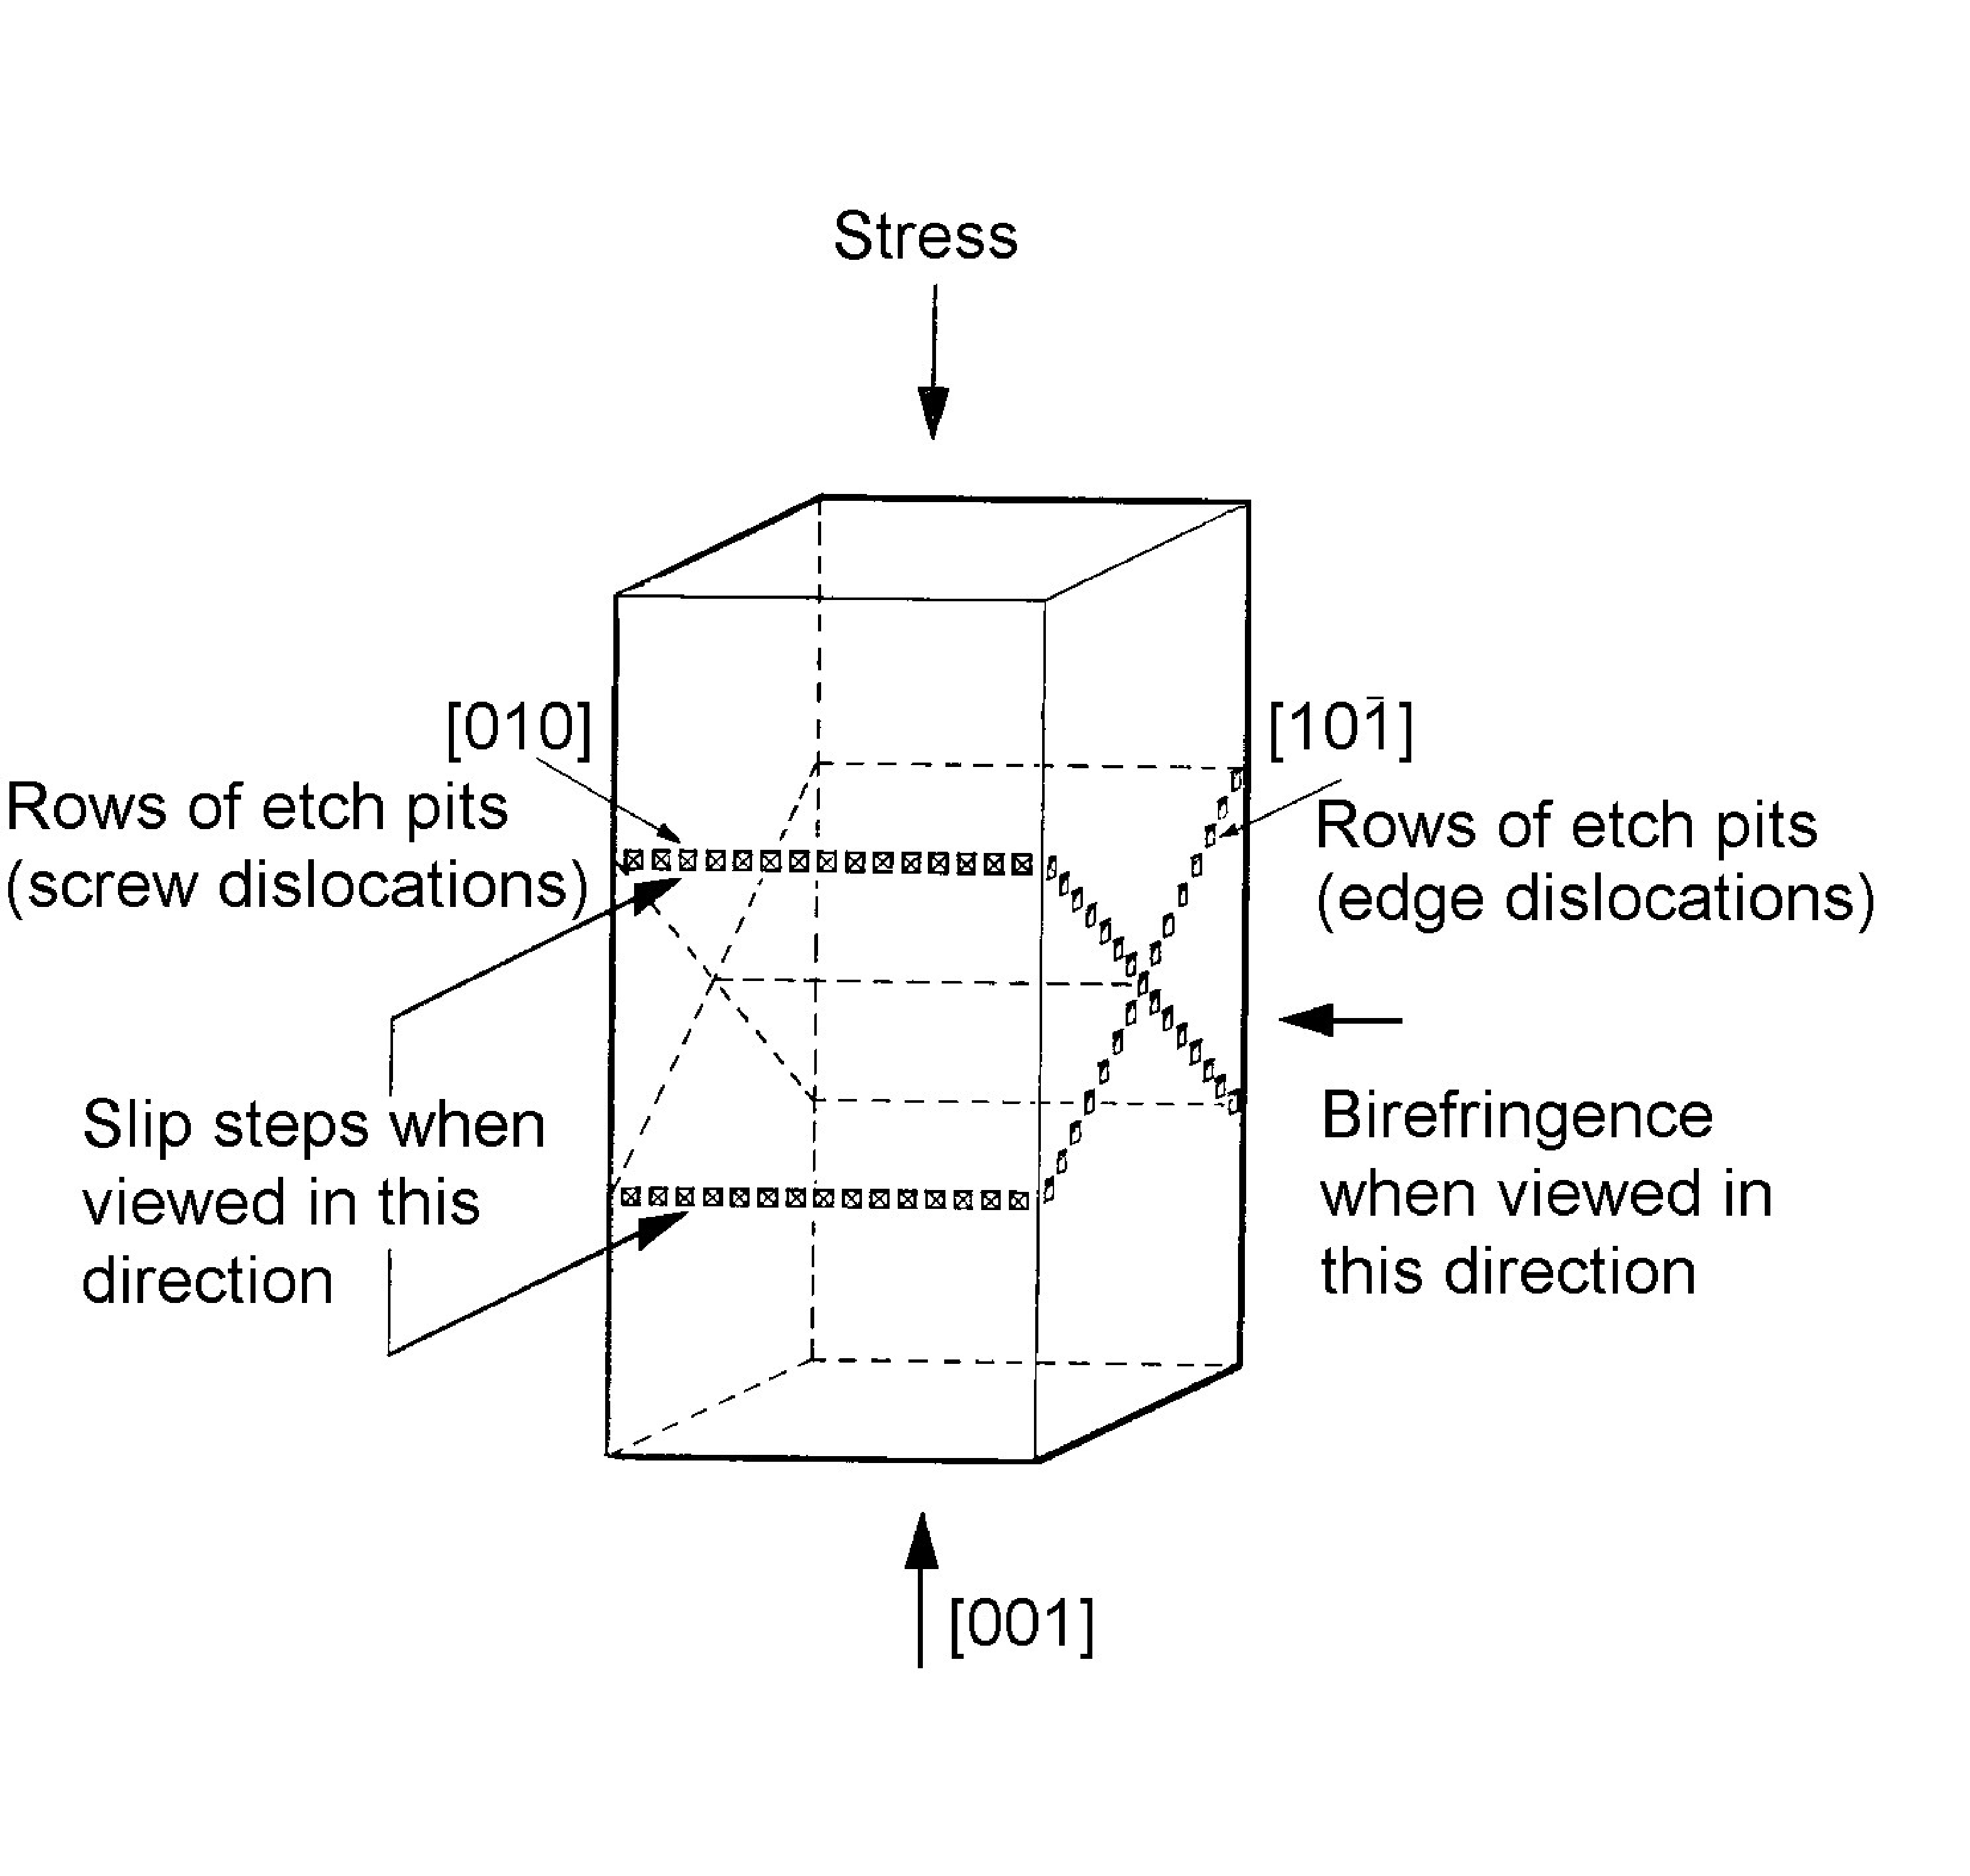
\includegraphics{Dislocations-Fig_19.pdf}
\caption{Quelle 1, S. 17}
\end{figure}

\hypertarget{winkel-zwischen-uxe4tzgruxfcbchen}{%
\subsection{Winkel zwischen
Ätzgrübchen}\label{winkel-zwischen-uxe4tzgruxfcbchen}}

Für den Winkel zwischen den Kristalliten \(\theta\), die in einer
Korngrenze aufeinander treffen, lässt sich geometrisch folgender
Zusammenhang zum Abstand \(d\) zweier Ätzgrübchen und dem Betrag \(b\)
des Burgers-Vektors finden.

\[
\begin{eqnarray}
    \sin(\theta) &=& \frac{b}{d}
\end{eqnarray}
\] Ist die Korngrenze eine Kleinwinkelkorngrenze
(\(\theta < 15^\circ\)), so lässt sich die Kleinwinkelnäherung für den
Sinus nutzen.

\[
\begin{eqnarray}
    \sin(\theta) &\approx& \theta \\
    \Rightarrow \theta &\approx& \frac{b}{d}
\end{eqnarray}
\] Der wahrscheinlichste Burgers-Vektor \(\vec{b}\) für \(\mathrm{LiF}\)
ist wie beschrieben der Vektor \([\frac{1}{2}\,0\,\frac{1}{2}]\) mit
einer Länge von \(b = \frac{a}{\sqrt{2}}\). \[
\begin{eqnarray}
    \theta &\approx& \frac{a}{\sqrt{2} \cdot d} \\
        &=& \frac{0.402\,\mathrm{nm}}{\sqrt{2} d}\\
    \theta &\approx& \frac{0.284\,\mathrm{nm}}{d} \label{theta}
\end{eqnarray}
\]

\hypertarget{durchfuxfchrung}{%
\section{Durchführung}\label{durchfuxfchrung}}

\hypertarget{vorbereitung-der-proben}{%
\subsection{Vorbereitung der Proben}\label{vorbereitung-der-proben}}

Eine Probe \(\mathrm{LiF}\)-Kristall mit äußeren Abmessungen von etwa
\(15 \times 3 \times 3 \,\mathrm{mm^3}\) wird zur Verfügung gestellt. Es
wurde zuvor von einem größeren Kristall durch Spalten abgetrennt und
dann für \(48\) Stunden bei \(650\,^\circ\mathrm C\) getempert und
langsam abgekühlt.

Eine zweite wird zu Beginn des Versuchs von einem größeren Block
abgespalten. Diese wird nicht getempert, allerdings chemisch poliert und
geätzt. Das Abspalten erfolgt mit einem Beitel, der parallel zu einer
Seitenfläche des großen Blocks angesetzt wird.

\hypertarget{polieren-und-uxe4tzen}\) aus
Tetrafluoroborsäure \((\mathrm{HBF_4})\), zu \(30\,\mathrm{Vol\%}\) aus
Salpetersäure \((\mathrm{HNO_3})\) und zu \(60\,\mathrm{Vol\%}\) aus
Wasser \((\mathrm{H_2O})\). Das Ätzmittel ist \(50\,\mathrm{ppm}\)
Eisen(III)-Chlorid \((\mathrm{FeCl_3})\) in destiliertem Wasser.

Beide Proben wurden für \(19\mathrm{\,min}\) in das Poliermittel
gegeben. Nach \(13.5\mathrm{\,min}\) wurden sie umgedreht, sodass alle
Seiten poliert wurden. Daraufhin wurden sie mit Ethanol abgespült,
jeweils \(6.5\mathrm{\,min}\) geätzt und wiederum mit Ethanol abgespült.

\hypertarget{uxe4tzgruxfcbchendichten-kleinwinkelkorngrenzen}{%
\subsection{Ätzgrübchendichten \&
Kleinwinkelkorngrenzen}\label{uxe4tzgruxfcbchendichten-kleinwinkelkorngrenzen}}

Daraufhin wurden die Proben daraufhin untersucht, welche Seite die
wenigsten Schäden und Stufen hat. Diese Seite wurde jeweils für die
folgenden Messungen verwendet.

Daraufhin wurden je Probe zwei Aufnahmen aufgenommen, auf denen
Ätzgrübchen erkennbar sind. Bei der getemperten Probe wurden je eine
Aufnahme bei \(2000\)-facher und bei \(1000\)-facher Vergrößerung
gemacht, bei der ungetemperten Probe je eine Aufnahme bei
\(1000\)-facher und \(500\)-facher Vergrößerung.

Dann wurden drei Kleinwinkelkorngrenzen auf der getemperten Probe
gesucht und bei \(2000\)-facher Vergrößerung vermessen. Hierzu wurden
jeweils \(4\) bis \(6\) Ätzgrübchen abgezählt.

\hypertarget{nadeldruckrosetten}{%
\subsection{Nadeldruckrosetten}\label{nadeldruckrosetten}}

Auf der getemperten Probe wurden an drei möglichst defektfreien Stellen
Eindrücke mit einer Nadel gemacht. Daraufhin wurde die Probe erneut für
\(6\mathrm{\,min}\) geätzt und danach mit Ethanol abgespült.

Die dabei entstandenen Rosetten wurden fotografiert. Dazu wurde zunächst
eine Übersicht bei \(50\)-facher Vergrößerung aufgenommen und dann
Einzelaufnahmen bei \(200\)- bzw. \(150\)-fachen Vergrößerungen
aufgenommen. Hierbei fiel direkt auf, dass die Rosette im Zentrum der
Probe größere Ausmaße hatte, weswegen eine geringere Vergrößerung als
für die anderen beiden Rosetten notwendig war, um die gesamte Rosette
abzubilden.

\hypertarget{eingespannte-probe}{%
\subsection{Eingespannte Probe}\label{eingespannte-probe}}

Nun wurde die Probe hochkant so in eine Presse eingespannt, dass die
vermessene Seite senkrecht war. Die Spannung wurde durch ein
Gesamtgewicht von \(1.789\mathrm{\,kg}\) erzeugt, das durch die obere
Hälfte der Presse und ein Zusatzgewicht von \(841\mathrm{\,g}\) erzeugt
wurde.

Nach \(2\mathrm{\,min}\) wurde die Probe herausgeholt und erneut für
\(6\mathrm{\,min}\) geätzt. Nach erneuten Abspülen mit Ethanol wurden
die Rosetten erneut fotografiert. Hierbei wurde darauf geachtet, dass
sowohl alte Ätzgrübchen als auch durch Wandern neu entstandene
Ätzgrübchen auf den Fotos sichtbar waren. Dies lässt sich durch die
Größe und Form der Ätzgrübchen unterscheiden.

Zuletzt wurde eingespannte Fläche vermessen. Dazu wurde die Probe
senkrecht auf das Mikroskop gestellt, sodass die Orientierung der Probe
der Orientierung beim Einspannen entsprach. Mithilfe des Mikroskops
wurde die Oberfläche der Probenschmalseite vermessen.

\hypertarget{auswertung}{%
\section{Auswertung}\label{auswertung}}

\hypertarget{uxe4tzgruxfcbchendichte}{%
\subsubsection{Ätzgrübchendichte}\label{uxe4tzgruxfcbchendichte}}

\hypertarget{berechnung}{%
\paragraph{Berechnung}\label{berechnung}}

Die Ätzgrübchendichte ist an verschiedene Stellen der jeweiligen Proben
sehr unterschiedlich, da durch die Ätzgrübchendichte lokale Unebenheiten
dargestellt werden.

Um die insgesamte Ätzgrübchendichte der beiden Proben abzuschätzen,
wurden für jede Probe an zwei repräsentativen Stellen Ätzgrübchen
aufgenommen, wobei die Ätzgrübchendichte \(N\) durch die Anzahl \(n\)
der Ätzgrübchen und die Fläche \(F\) bestimmt ist. Die Ungenauigkeit
\(\Delta N\) der Ätzgrübchendichte ist nach Gauß'scher
Fehlerfortpflanzung zu bestimmen.

\[
\begin{eqnarray}
    N &=& \frac{n}{F} \label{N}\\
    \Delta N &=& \sqrt{
        \left(\frac{\Delta n}{F}\right)^2
        + \left(\frac{n}{F^2} \cdot \Delta F\right)^2} \label{DeltaN}
\end{eqnarray}
\]

Der Fehler der Anzahl der Ätzgrübchendichte \(\Delta n\) hängt neben
menschlicher Ablesefähigkeit auch von der Schärfe des jeweiligen Bildes
ab. Wir schätzen ihn dennoch für alle Bilder auf \(10\,\%\), da in
unserem Fall die Bilder mit höherer Unschärfe auch die kleinere Anzahl
an Ätzgrübchen haben. Der Fehler der Fläche \(\Delta F\) ist durch die
Genauigkeit der Streckenangabe des Mikroskops gegeben und beträgt
\(\Delta F=(0.005 \mathrm{\, \mu m})^2\).

Um die durchschnittliche Ätzgrübchendichte der Proben zu bestimmen,
nehmen wir den Mittelwert der Dichten an den zwei Stellen, die
Ungenauigkeit ist durch die Standardabweichung gegeben.

\[
\begin{eqnarray}
    \bar{N} &=& \frac{N_1 + N_2}{2} \label{Nbar}\\
    \Delta \bar N &=& \left| \frac{N_1 - N_2}{2} \right| \label{DeltaNbar}
\end{eqnarray}
\]

\hypertarget{nicht-getemperte-probe}{%
\paragraph{Nicht-getemperte Probe}\label{nicht-getemperte-probe}}

Wie in Abbildung \(1??\) zu sehen, sind in den inneren sechs blauen
Quadraten insgesamt \(5\pm1\) Ätzgrübchen zu finden, die Quadrate haben
jeweils eine Seitenlänge von \(200.00 \mathrm{\,\mu m}\).

An der zweiten Stelle der nicht getemperten Probe (siehe Abbildung
\(2??\)) sind in den inneren sechs blauen Quadraten \(16\pm1\)
Ätzgrübchen zu finden, die Quadrate hier je eine Seitenlänge von
\(100.00 \mathrm{\, \mu m}\).

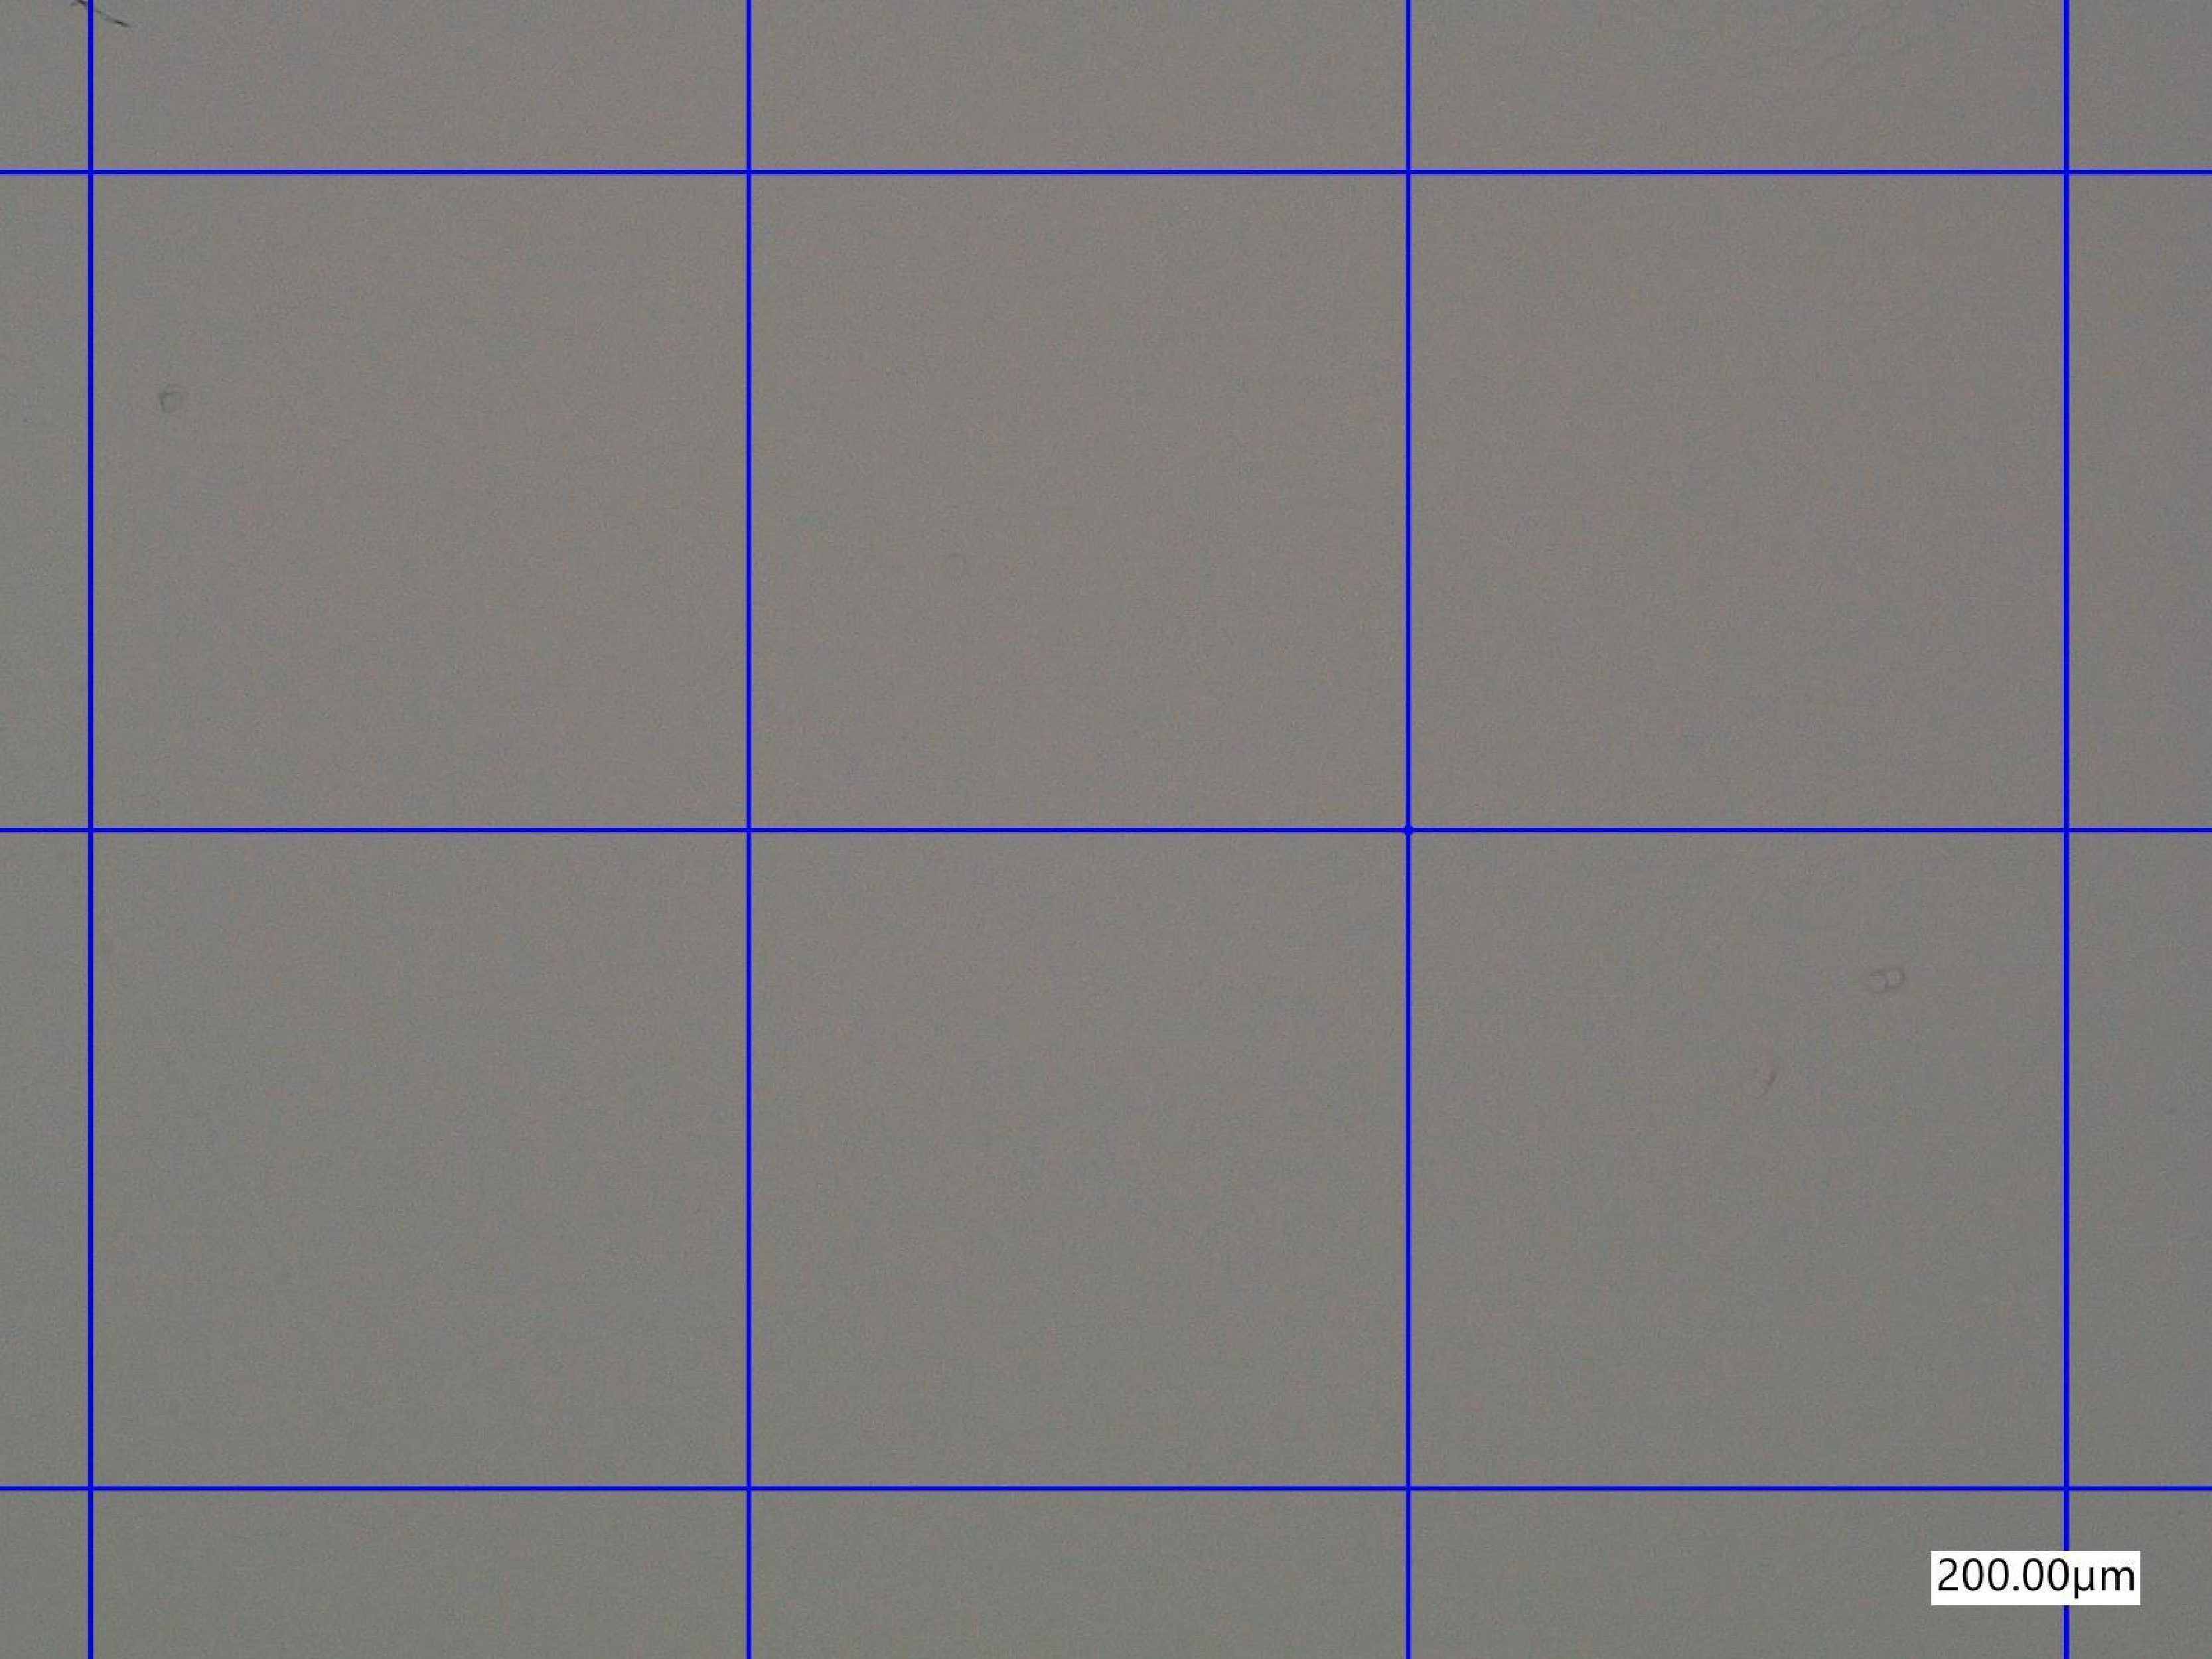
\includegraphics{Dichte1_not_tempered.pdf}
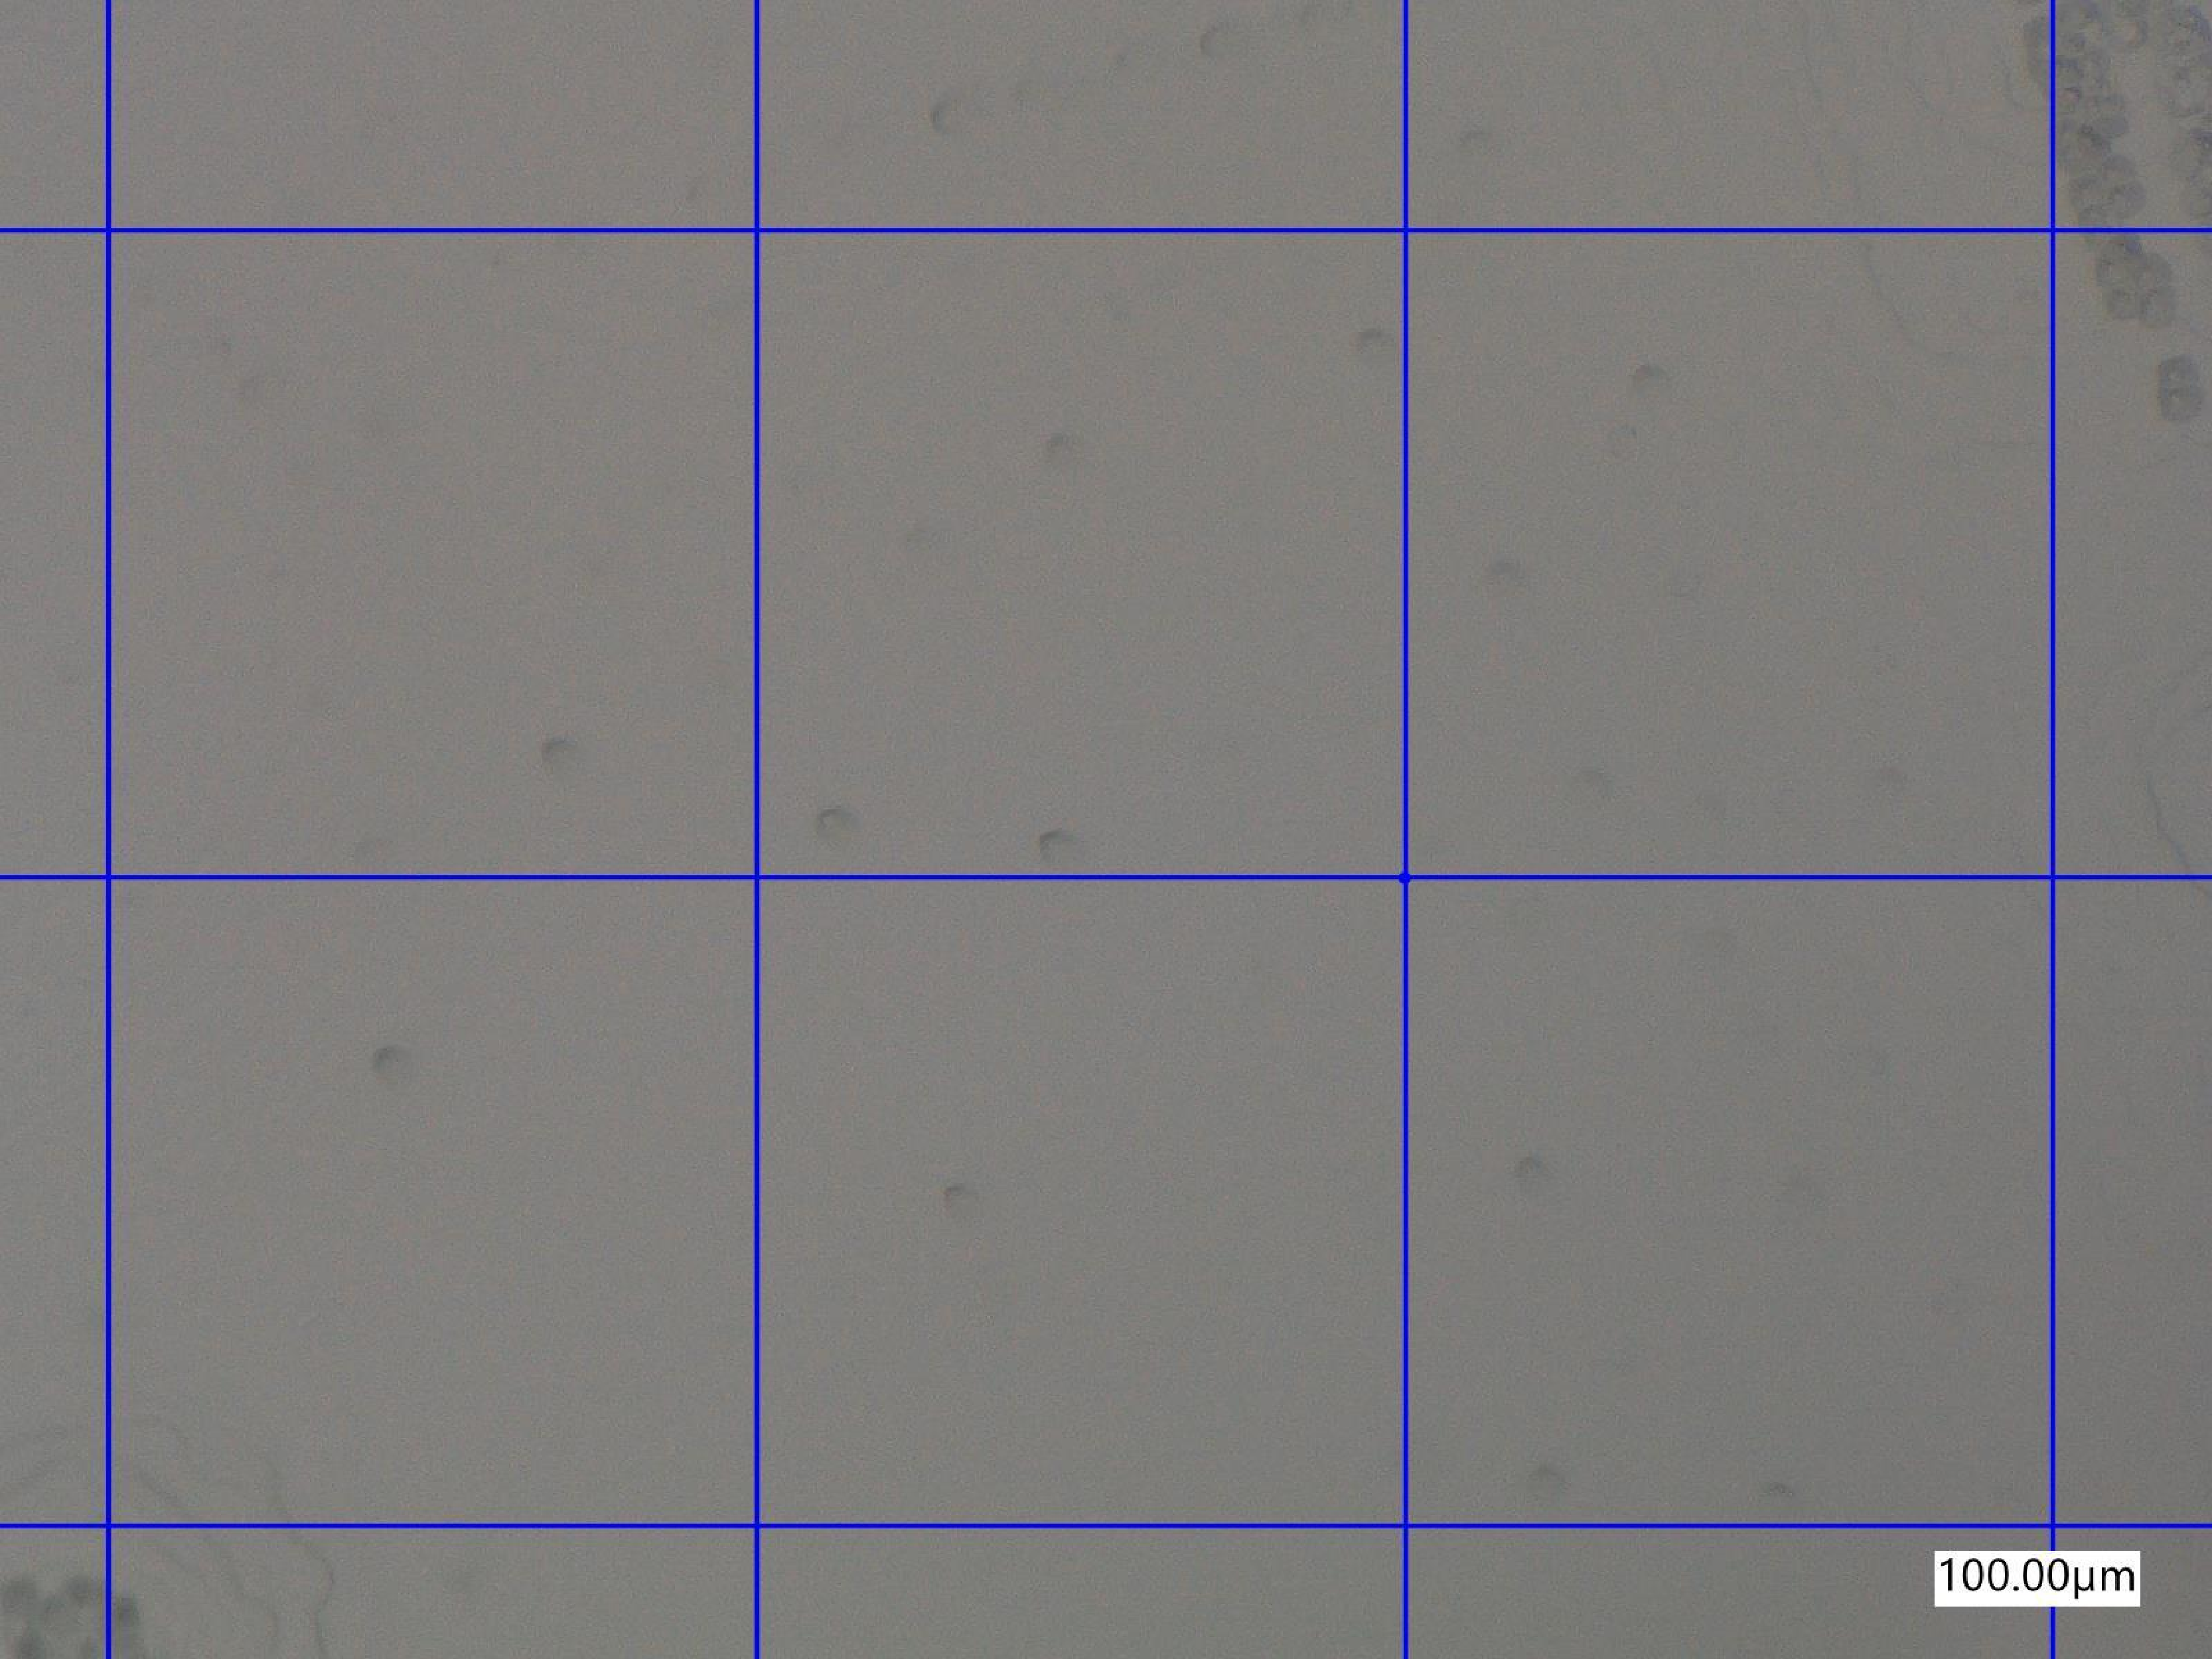
\includegraphics{Dichte2_not_tempered.pdf}

Mithilfe der Gleichungen \(\eqref{N}\) bis \(\eqref{DeltaNbar}\) folgt
die mittlere Ätzgrübchendichte \(\bar N_\mathrm{nt}\) der
nicht-getemperten Probe.

\[
\begin{eqnarray}
    N_\mathrm{nt,1} &=& (2.1 \pm 0.4) \cdot 10^3 \mathrm{\, cm^{-2}} \\
    N_\mathrm{nt,2} &=& (2.7 \pm 0.3) \cdot 10^{4} \mathrm{\, cm^{-2}} \\
    \bar N_\mathrm{nt}
        &=& (1.4 \pm 1.2) \cdot 10^4 \mathrm{\, cm^{-2}}
        \quad(\pm 85.52\,\%)
\end{eqnarray}
\]

\hypertarget{getemperte-probe}{%
\paragraph{getemperte Probe}\label{getemperte-probe}}

In Abbildung \(3??\) sind insgesamt \(50\) Ätzgrübchen in den inneren
acht blauen Quadraten zu entdecken. Jedes dieser Quadrate hat eine
Seitenlänge von \(150.00 \mathrm{\, \mu m}\).

Die zweite Stelle der getemperten Probe ist in Abbildung \(4??\) zu
sehen. Dort sind \(81\pm8\) Ätzgrübchen in den inneren zwölf blauen
Quadraten zu finden. Jedes der Quadrate hat eine Seitenlänge von
\(70.00 \mathrm{\, \mu m}\).

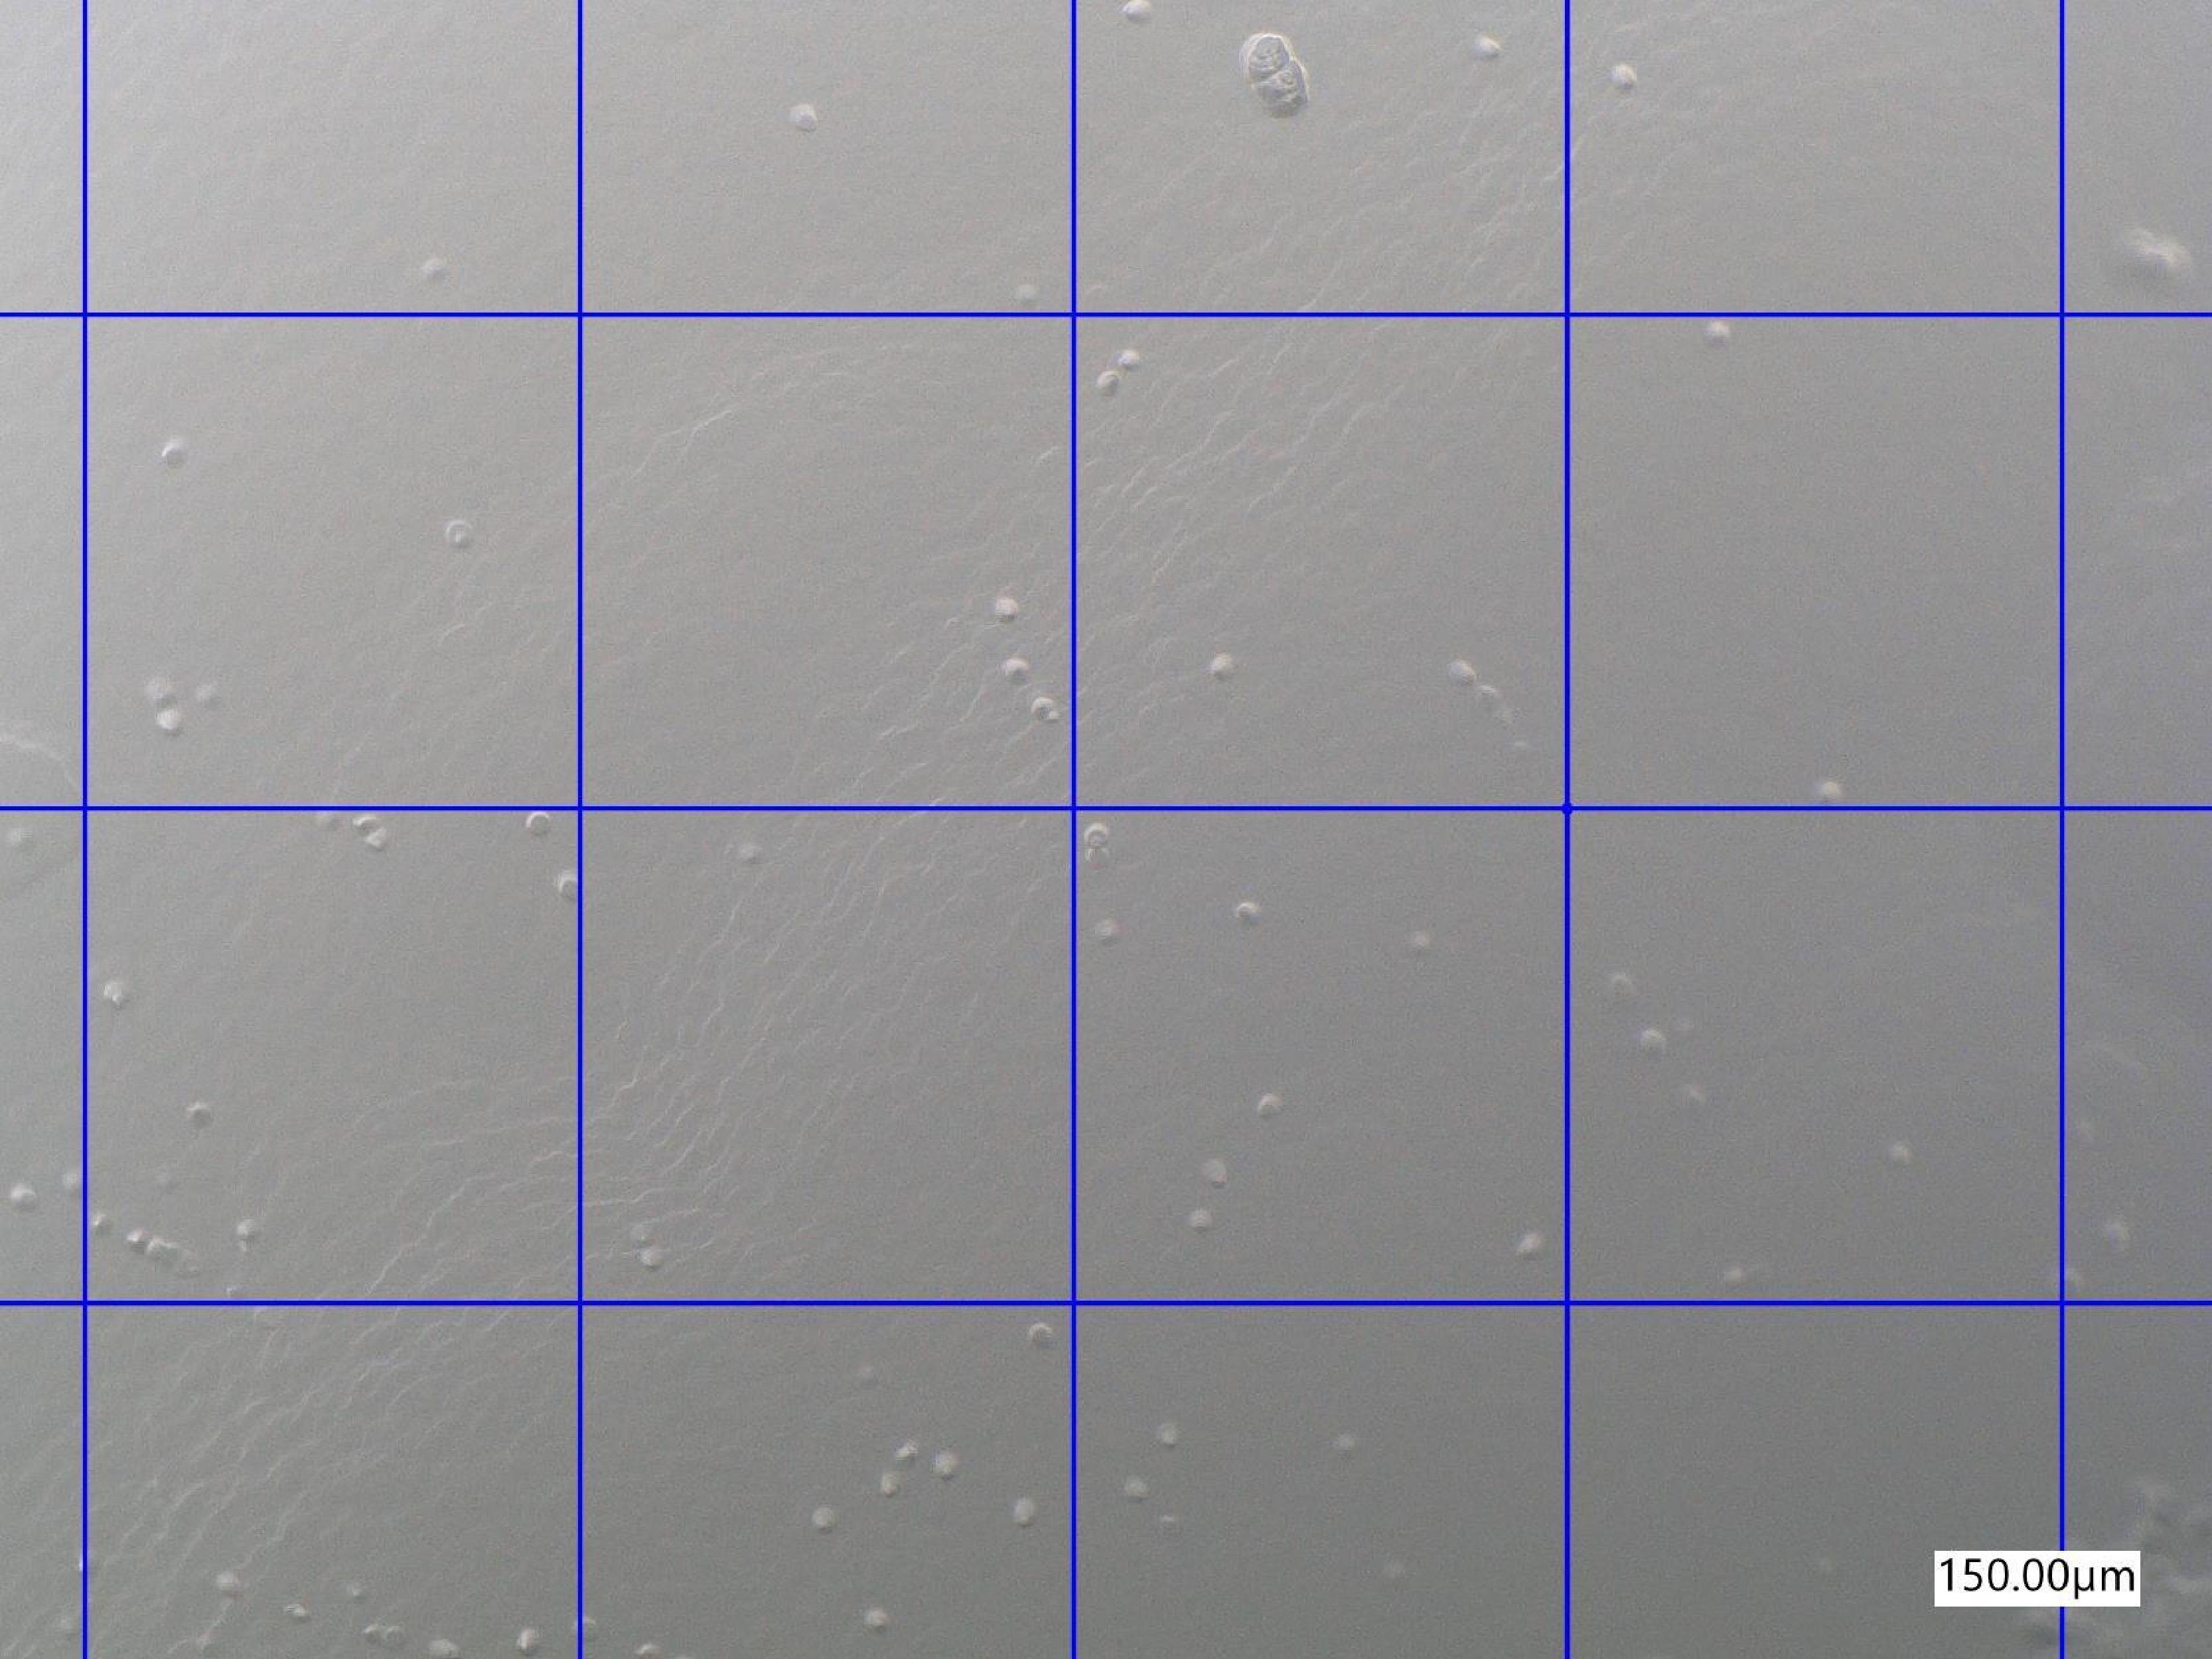
\includegraphics{Dichte1_tempered.pdf}
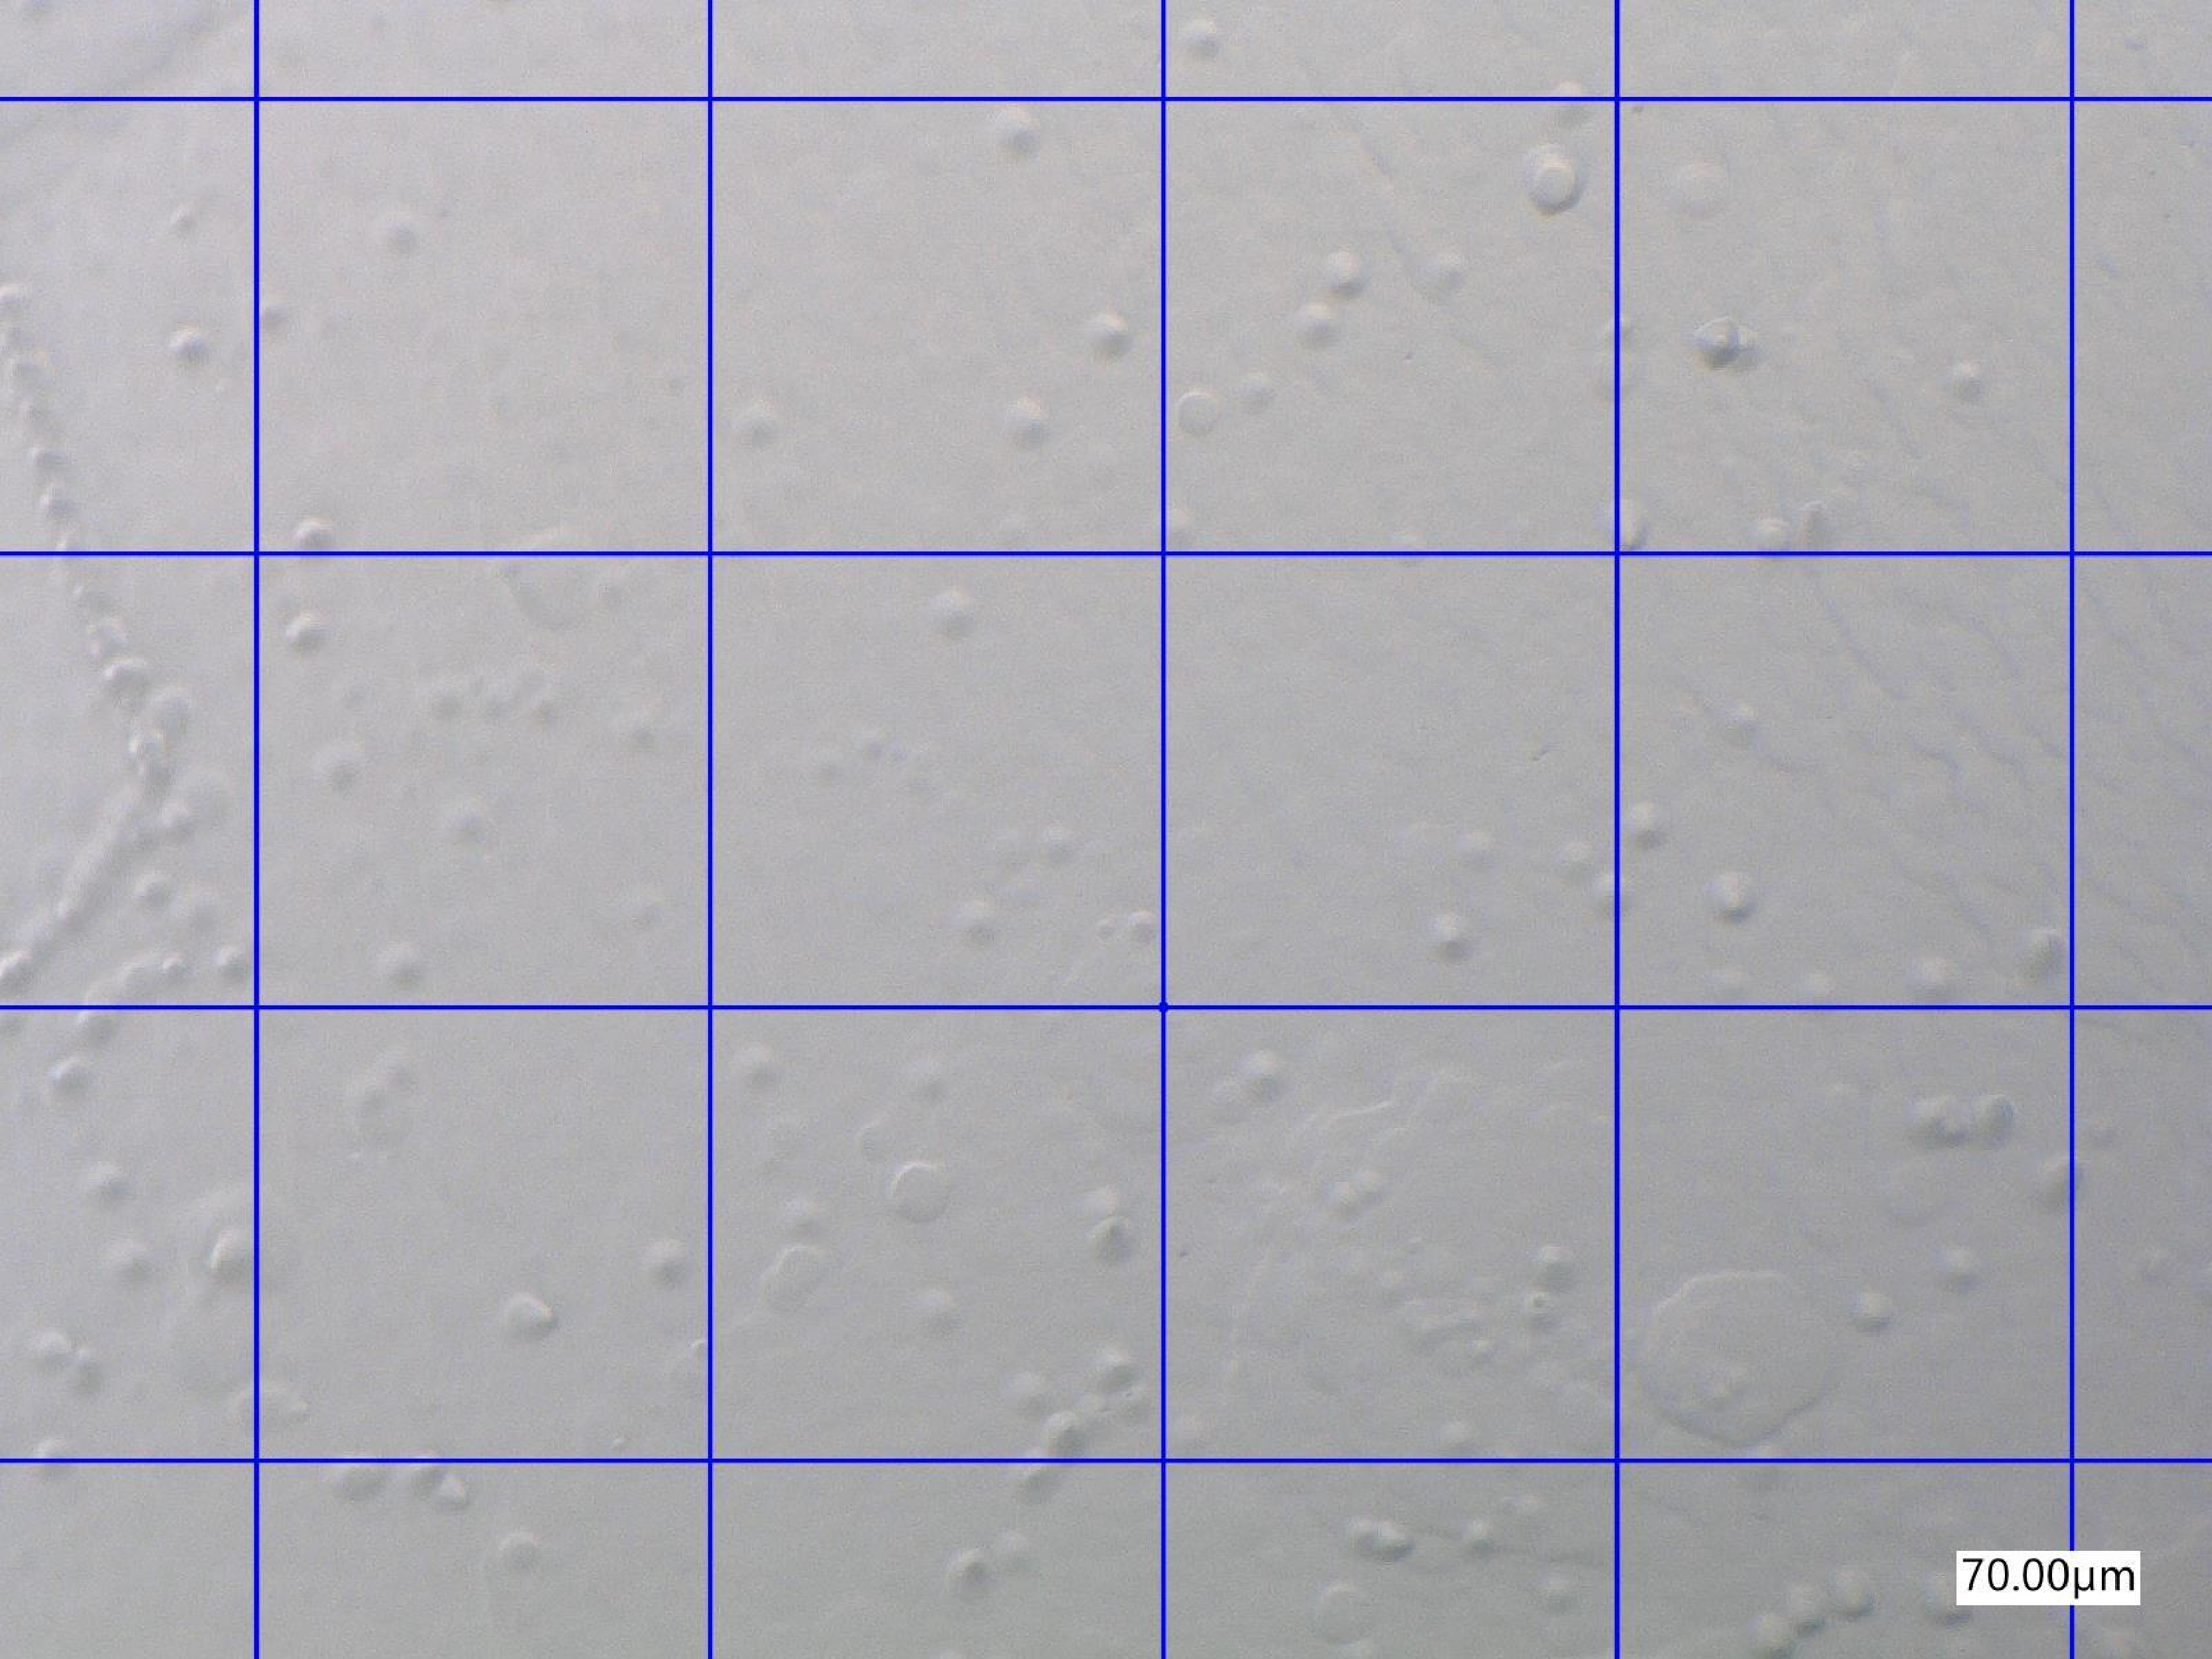
\includegraphics{Dichte2_tempered.pdf}

Wieder folgt aus den Gleichungen \(\eqref{N}\) bis \(\eqref{DeltaNbar}\)
die mittlere Ätzgrübchendichte \(\bar N_\mathrm{t}\) der getemperten
Probe.

\[
\begin{eqnarray}
    N_\mathrm{t,1} &=& (2.8 \pm 0.3) \cdot 10^4 \mathrm{\, cm^{-2}} \\
    N_\mathrm{t,2} &=& (1.4 \pm 0.1) \cdot 10^5 \mathrm{\, cm^{-2}}
    \\
    \bar N_\mathrm{t}
        &=& (8.3 \pm 5.5) \cdot 10^4 \mathrm{\, cm^{-2}}
        \quad(\pm 66.44\,\%)
\end{eqnarray}
\]

\hypertarget{diskussion}{%
\paragraph{Diskussion}\label{diskussion}}

Die großen Fehler in den Mittelwerten der Ätzgrübchendichten folgen
daraus, dass wir nur zwei typische Stellen pro Probe verwenden um die
durchschnittliche Ätzgrübchendichte der gesamten Probe zu bestimmen. Die
Ergebnisse sind trotzdem gut interpretierbar.

Eigentlich würden wir erwarten, dass die Ätzgrübchendichte und damit die
Versetzungsdichte der getemperten Probe niedriger ist als die der nicht
getemperten Probe, da sich die Versetzungen in der Probe beim
Temperungsprozess auslöschen. \([1]\)

Hier erhalten wir aber das Gegenteil. Die Ätzgrübchendichte der
getemperten Probe ist mit ca.
\(\bar N_\mathrm{t}=(8.3\pm 5.5) \cdot 10^4 \mathrm{\, cm^{-2}}\) selbst
innerhalb der Fehlergrenzen größer als die Ätzgrübchendichte der nicht
getemperten Probe
\(\bar N_\mathrm{nt}=(1.4 \pm 1.2) \cdot 10^4 \mathrm{\, cm^{-2}}\).

Dies kann mehrere Ursachen haben. Die erste Möglichkeit ist, dass unsere
ausgesuchten repräsentativen Stellen doch nicht so repräsentativ sind
wie wir dachten. Wir hätten z.B. aus Versehen eine oder beide Stellen
der getemperten Probe innerhalb einer stark beschädigten Zone wählen
können.

Dies führt direkt zur zweiten Möglichkeit. Es kann sein, dass die
getemperte Probe nach dem Tempern beschädigt wurde und so neue
Versetzungen hinzukamen.

In beiden Fällen ist das gemessene Ergebnis nicht undenkbar, wenn auch
unerwartet. Der Effekt des Temperns auf die Ätzgrübchendichte der Probe
konnte somit zwar nicht beobachtet werden. Dennoch konnte ein Gefühl für
die Menge an Versetzungen in \(\mathrm{LiF}\) entwickelt werden.

\hypertarget{kleinwinkelkorngrenze}{%
\subsubsection{Kleinwinkelkorngrenze}\label{kleinwinkelkorngrenze}}

Es wurden drei Bilder von Kleinwinkelkorngrenzen aufgenommen. Nun werden
die Winkel \(\theta\) zwischen den Kristalliten an diesen
Kleinwinkelkorngrenzen bestimmen. Dieser durch Gleichung
\(\eqref{theta}\) gegeben, wobei \(d\) den Abstand zweier Ätzgrübchen
beschreibt.

Die Ungenauigkeit der Gitterkonstante
\(\Delta a=1 \cdot 10^{-7} \mathrm{\, \mu m}\) \([5]\) und die des
Mikroskops \(\Delta d_m = 5 \cdot 10^{-3} \mathrm{\, \mu m}\) ergeben
mittels Gauß'scher Fehlerfortpflanzung die Ungenauigkeit des Winkels
\(\Delta \theta\). Wird der Abstand \(d_n\) von \(n\) Grübchen gemessen,
so sinkt die Ungenauigkeit \(\Delta d\) des Abstandes zweier Grübchen.

\[
\begin{eqnarray}
    \Delta d &=& \frac{\Delta d_m}{n} \\
    \Delta \theta &=& \sqrt{
        \left(\frac{\Delta a}{\sqrt{2} \cdot d} \right)^2
            + \left( \frac{a}{\sqrt{2} \cdot d^2} \cdot \Delta d \right)^2 }
            \label{DeltaTheta}
\end{eqnarray}
\]

\hypertarget{erste-messung}{%
\paragraph{erste Messung}\label{erste-messung}}

In Abbildung \(5??\) ist die erste Kleinwinkelkorngrenze zu sehen. In
rot ist der Abstand \(18.28 \mathrm{\, \mu m}\) für \(5\) Ätzgrübchen
eingetragen.

\begin{figure}
\centering
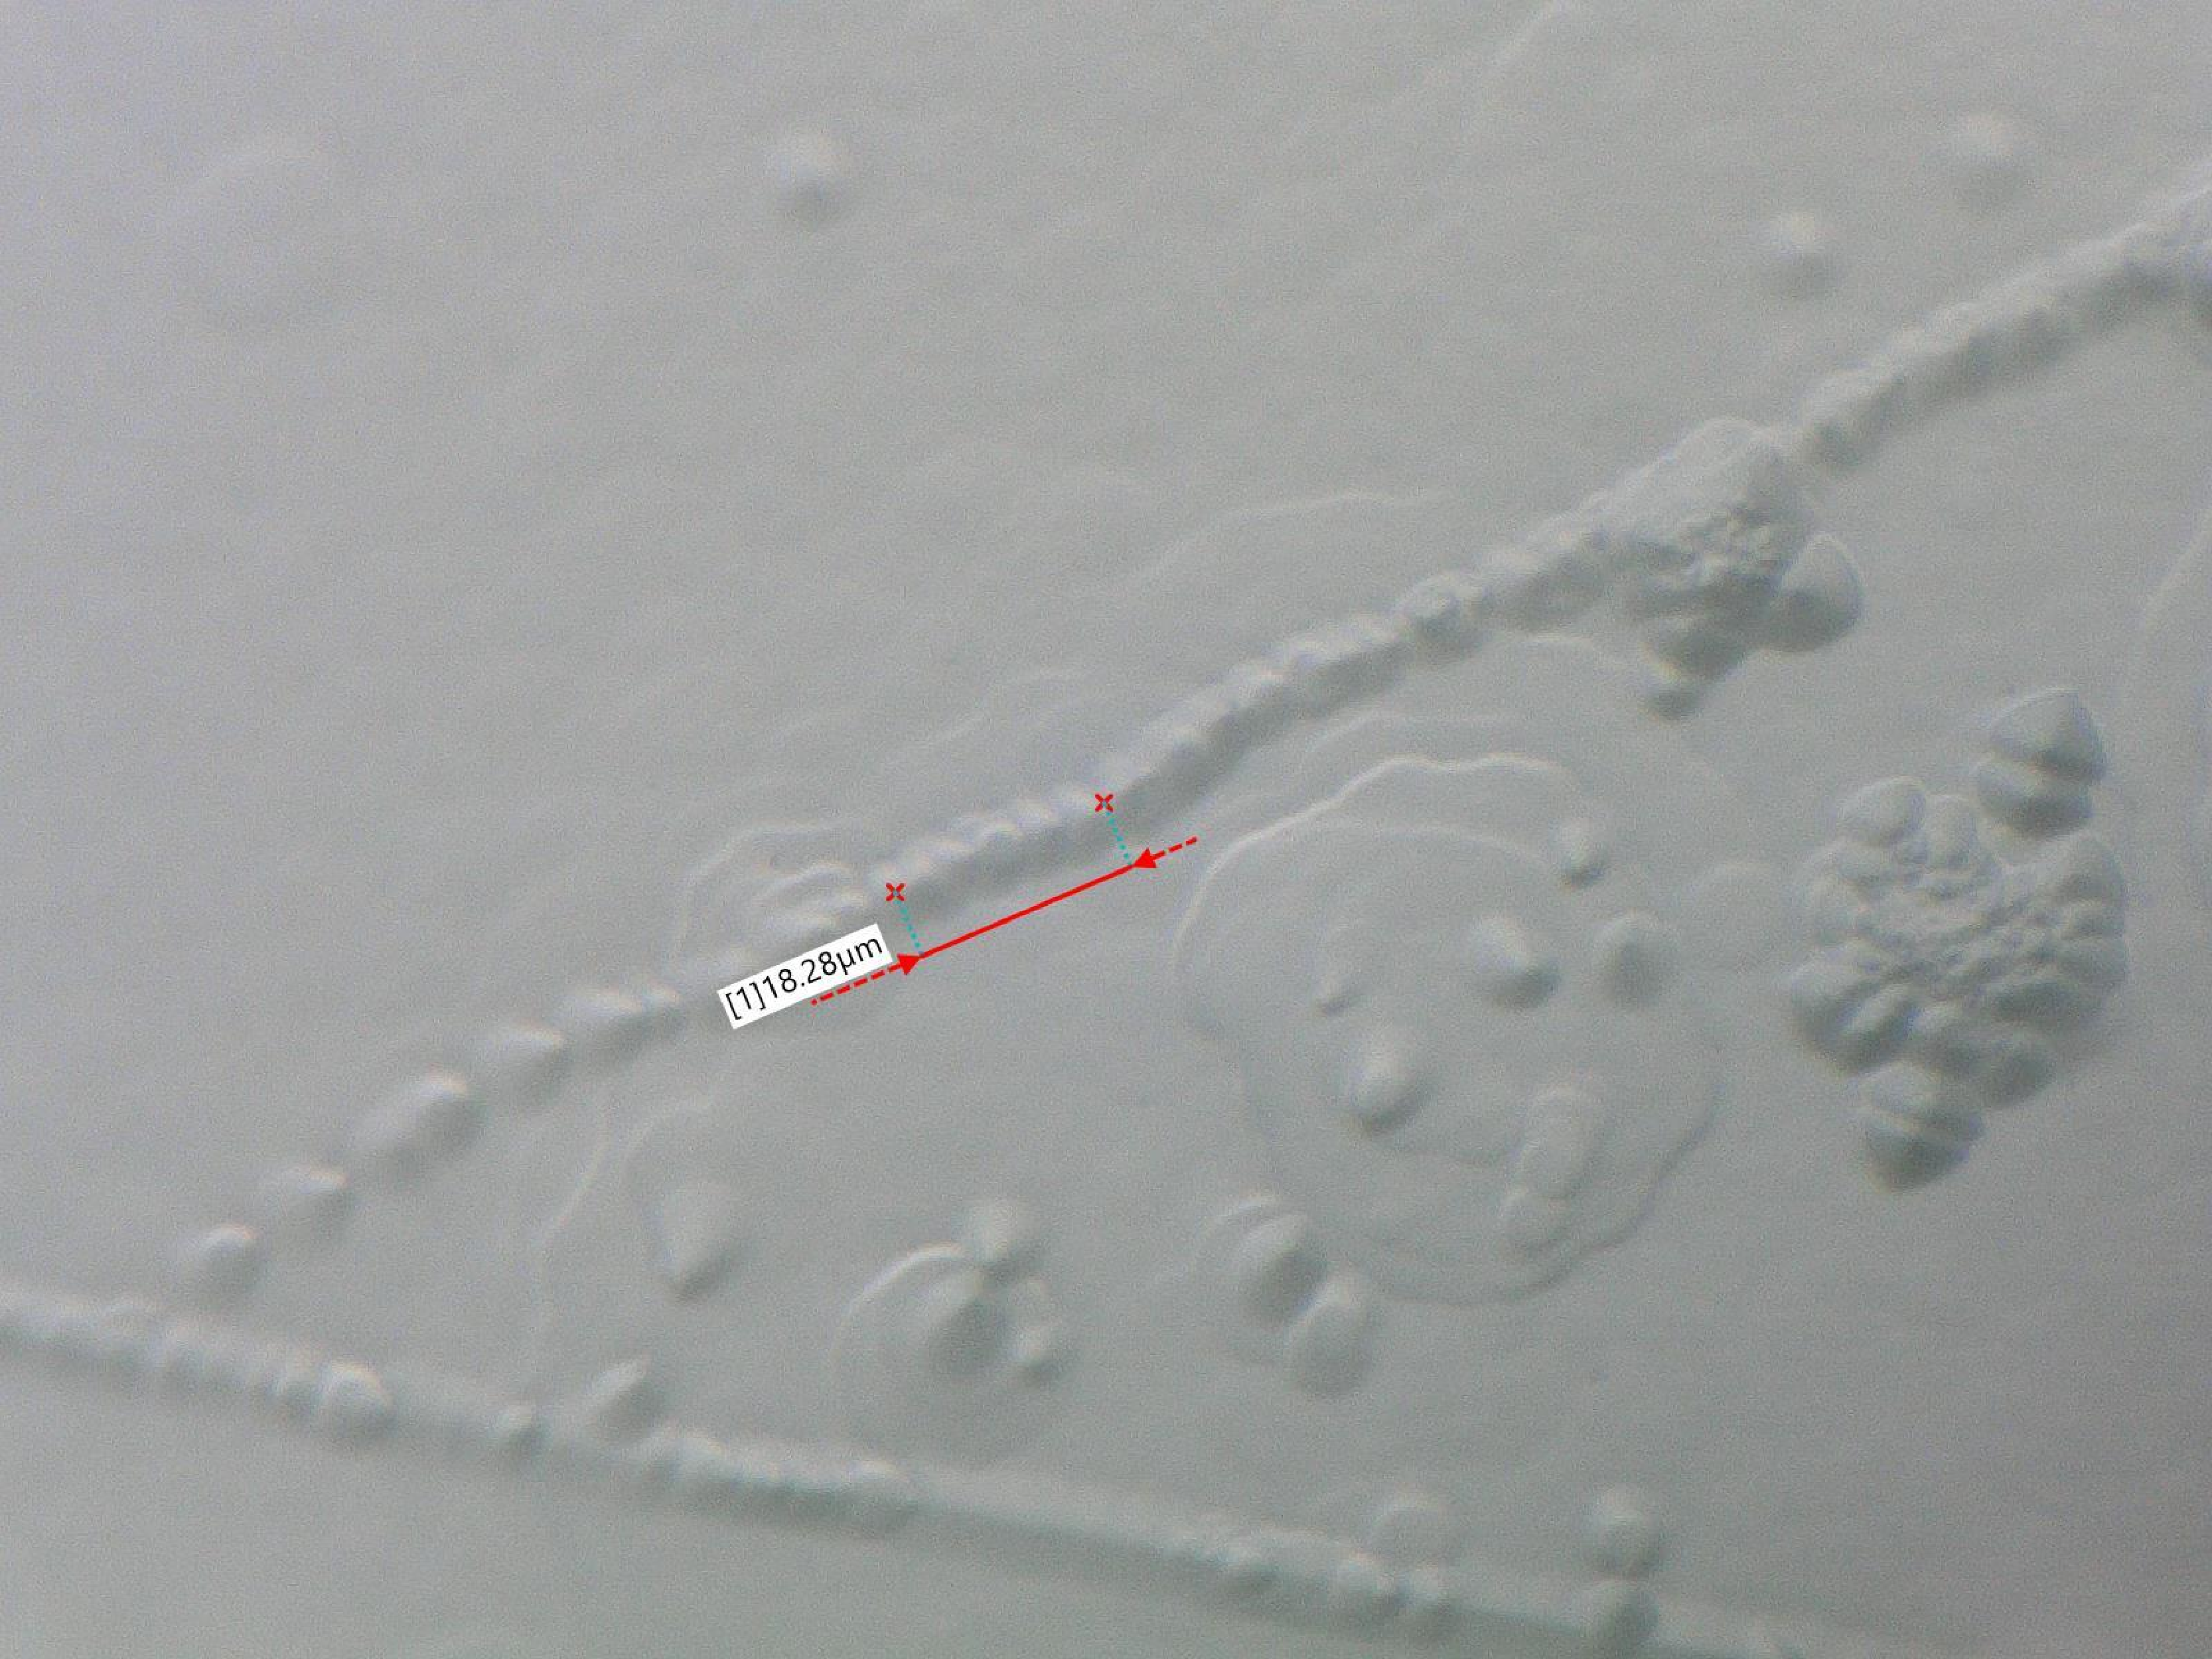
\includegraphics{KWK1_tempered.pdf}
\caption{Abb. 5}
\end{figure}

Aus \(\eqref{theta}\) und \(\eqref{DeltaTheta}\) folgt der erste Abstand
\(d_1\), woraus der Winkel \(\theta_1\) bestimmt wird.

\[
\begin{eqnarray}
    d_1 &=& (3.656 \pm 0.002) \mathrm{\, \mu m} \\
    \theta_1 &=& (7.775 \pm 0.005) \cdot 10^{-5} \mathrm{\, rad} \\
        &=& (4.455 \pm 0.003) \cdot 10^{-3\ \ \circ}
\end{eqnarray}
\]

\hypertarget{zweite-messung}{%
\paragraph{zweite Messung}\label{zweite-messung}}

Die zweite von uns aufgenommene Kleinwinkelkorngrenze ist in Abbildung
\(6\) zu sehen. Hier ist wieder der Abstand von \(5\) Ätzgrübchen mit
\(14.53 \mathrm{\, \mu m}\) eingetragen.

\begin{figure}
\centering
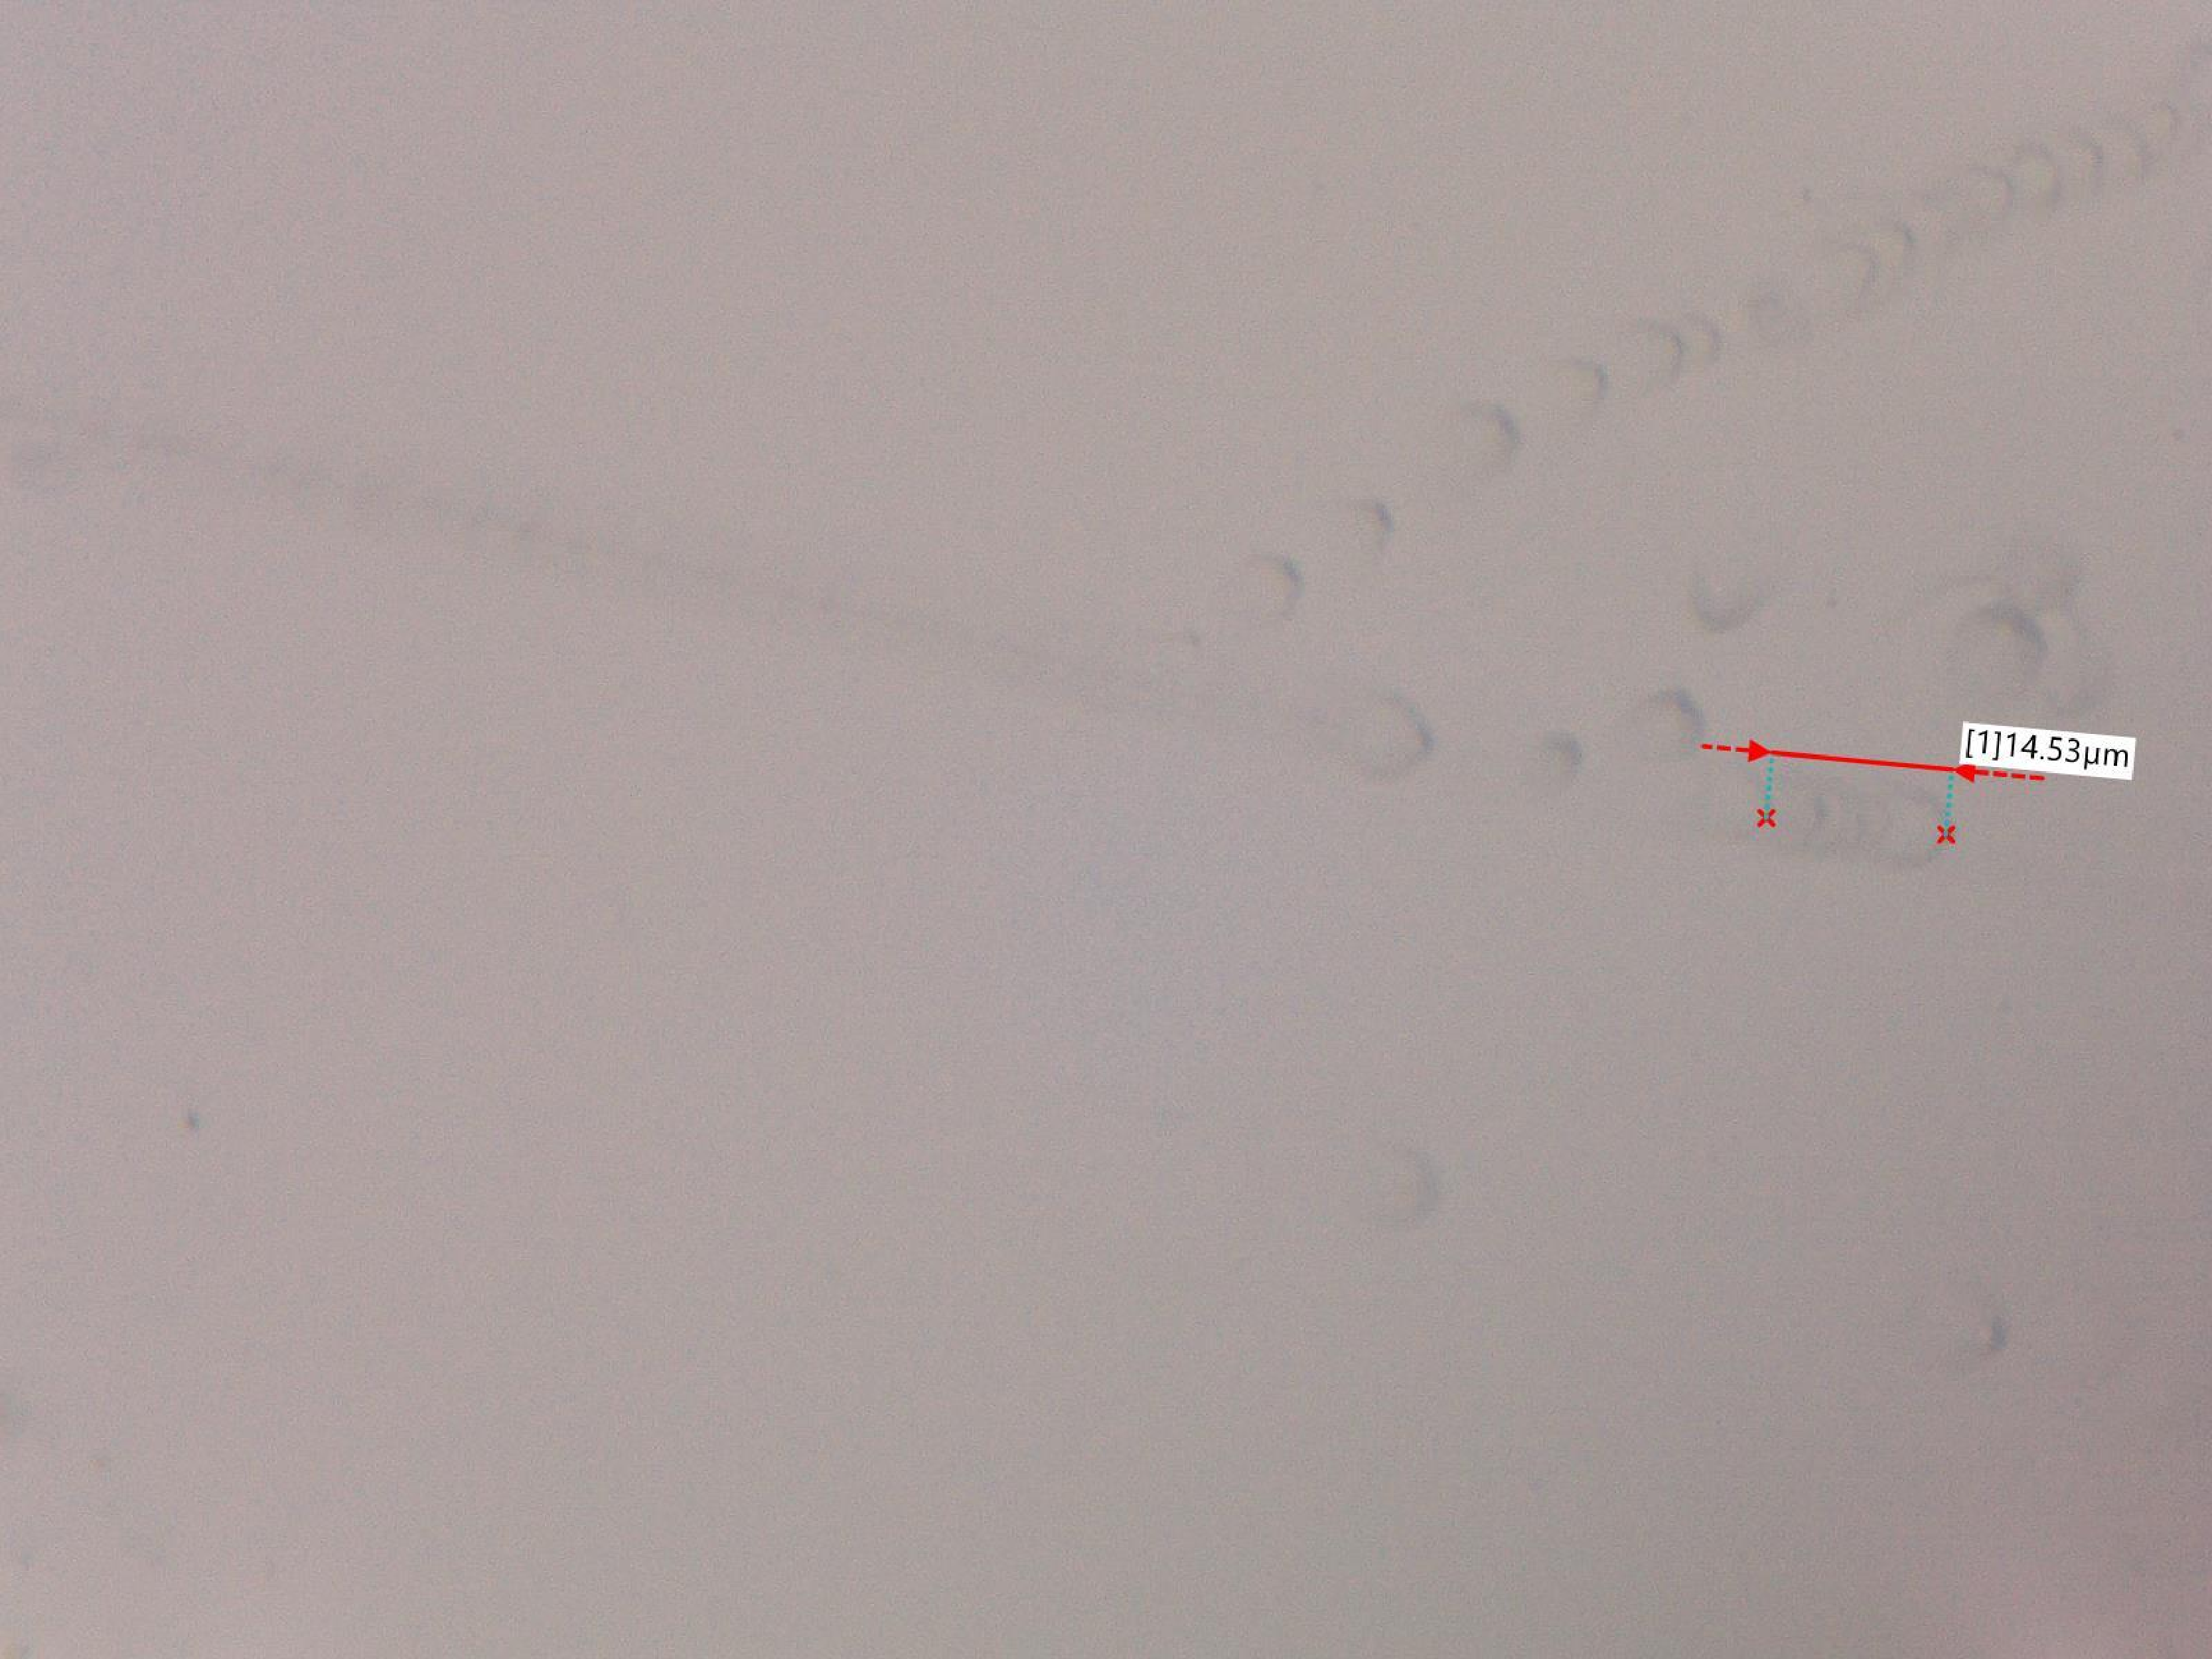
\includegraphics{KWK2_tempered.pdf}
\caption{Abb. 6}
\end{figure}

Der Abstand zweier Ätzgrübchen \(d_2\) sowie der Winkel \(\theta_2\)
werden analog bestimmt. \[
\begin{eqnarray}
    d_2 & = & (2.096\pm 0.002) \cdot 10^{-3} \mathrm{\, \mu m} \\
    \theta_2 &=& (9.782 \pm 0.008) \cdot 10^{-5} \mathrm{\, rad} \\
        &=& (5.605 \pm 0.005) \cdot 10^{-3\ \circ}
\end{eqnarray}
\]

\hypertarget{dritte-messung}{%
\paragraph{dritte Messung}\label{dritte-messung}}

An der letzten untersuchten Stelle ist der Abstand für \(3\) Ätzgrübchen
von \(16.76 \mathrm{\, \mu m}\) zu sehen, siehe Abb. \(7\).

\begin{figure}
\centering
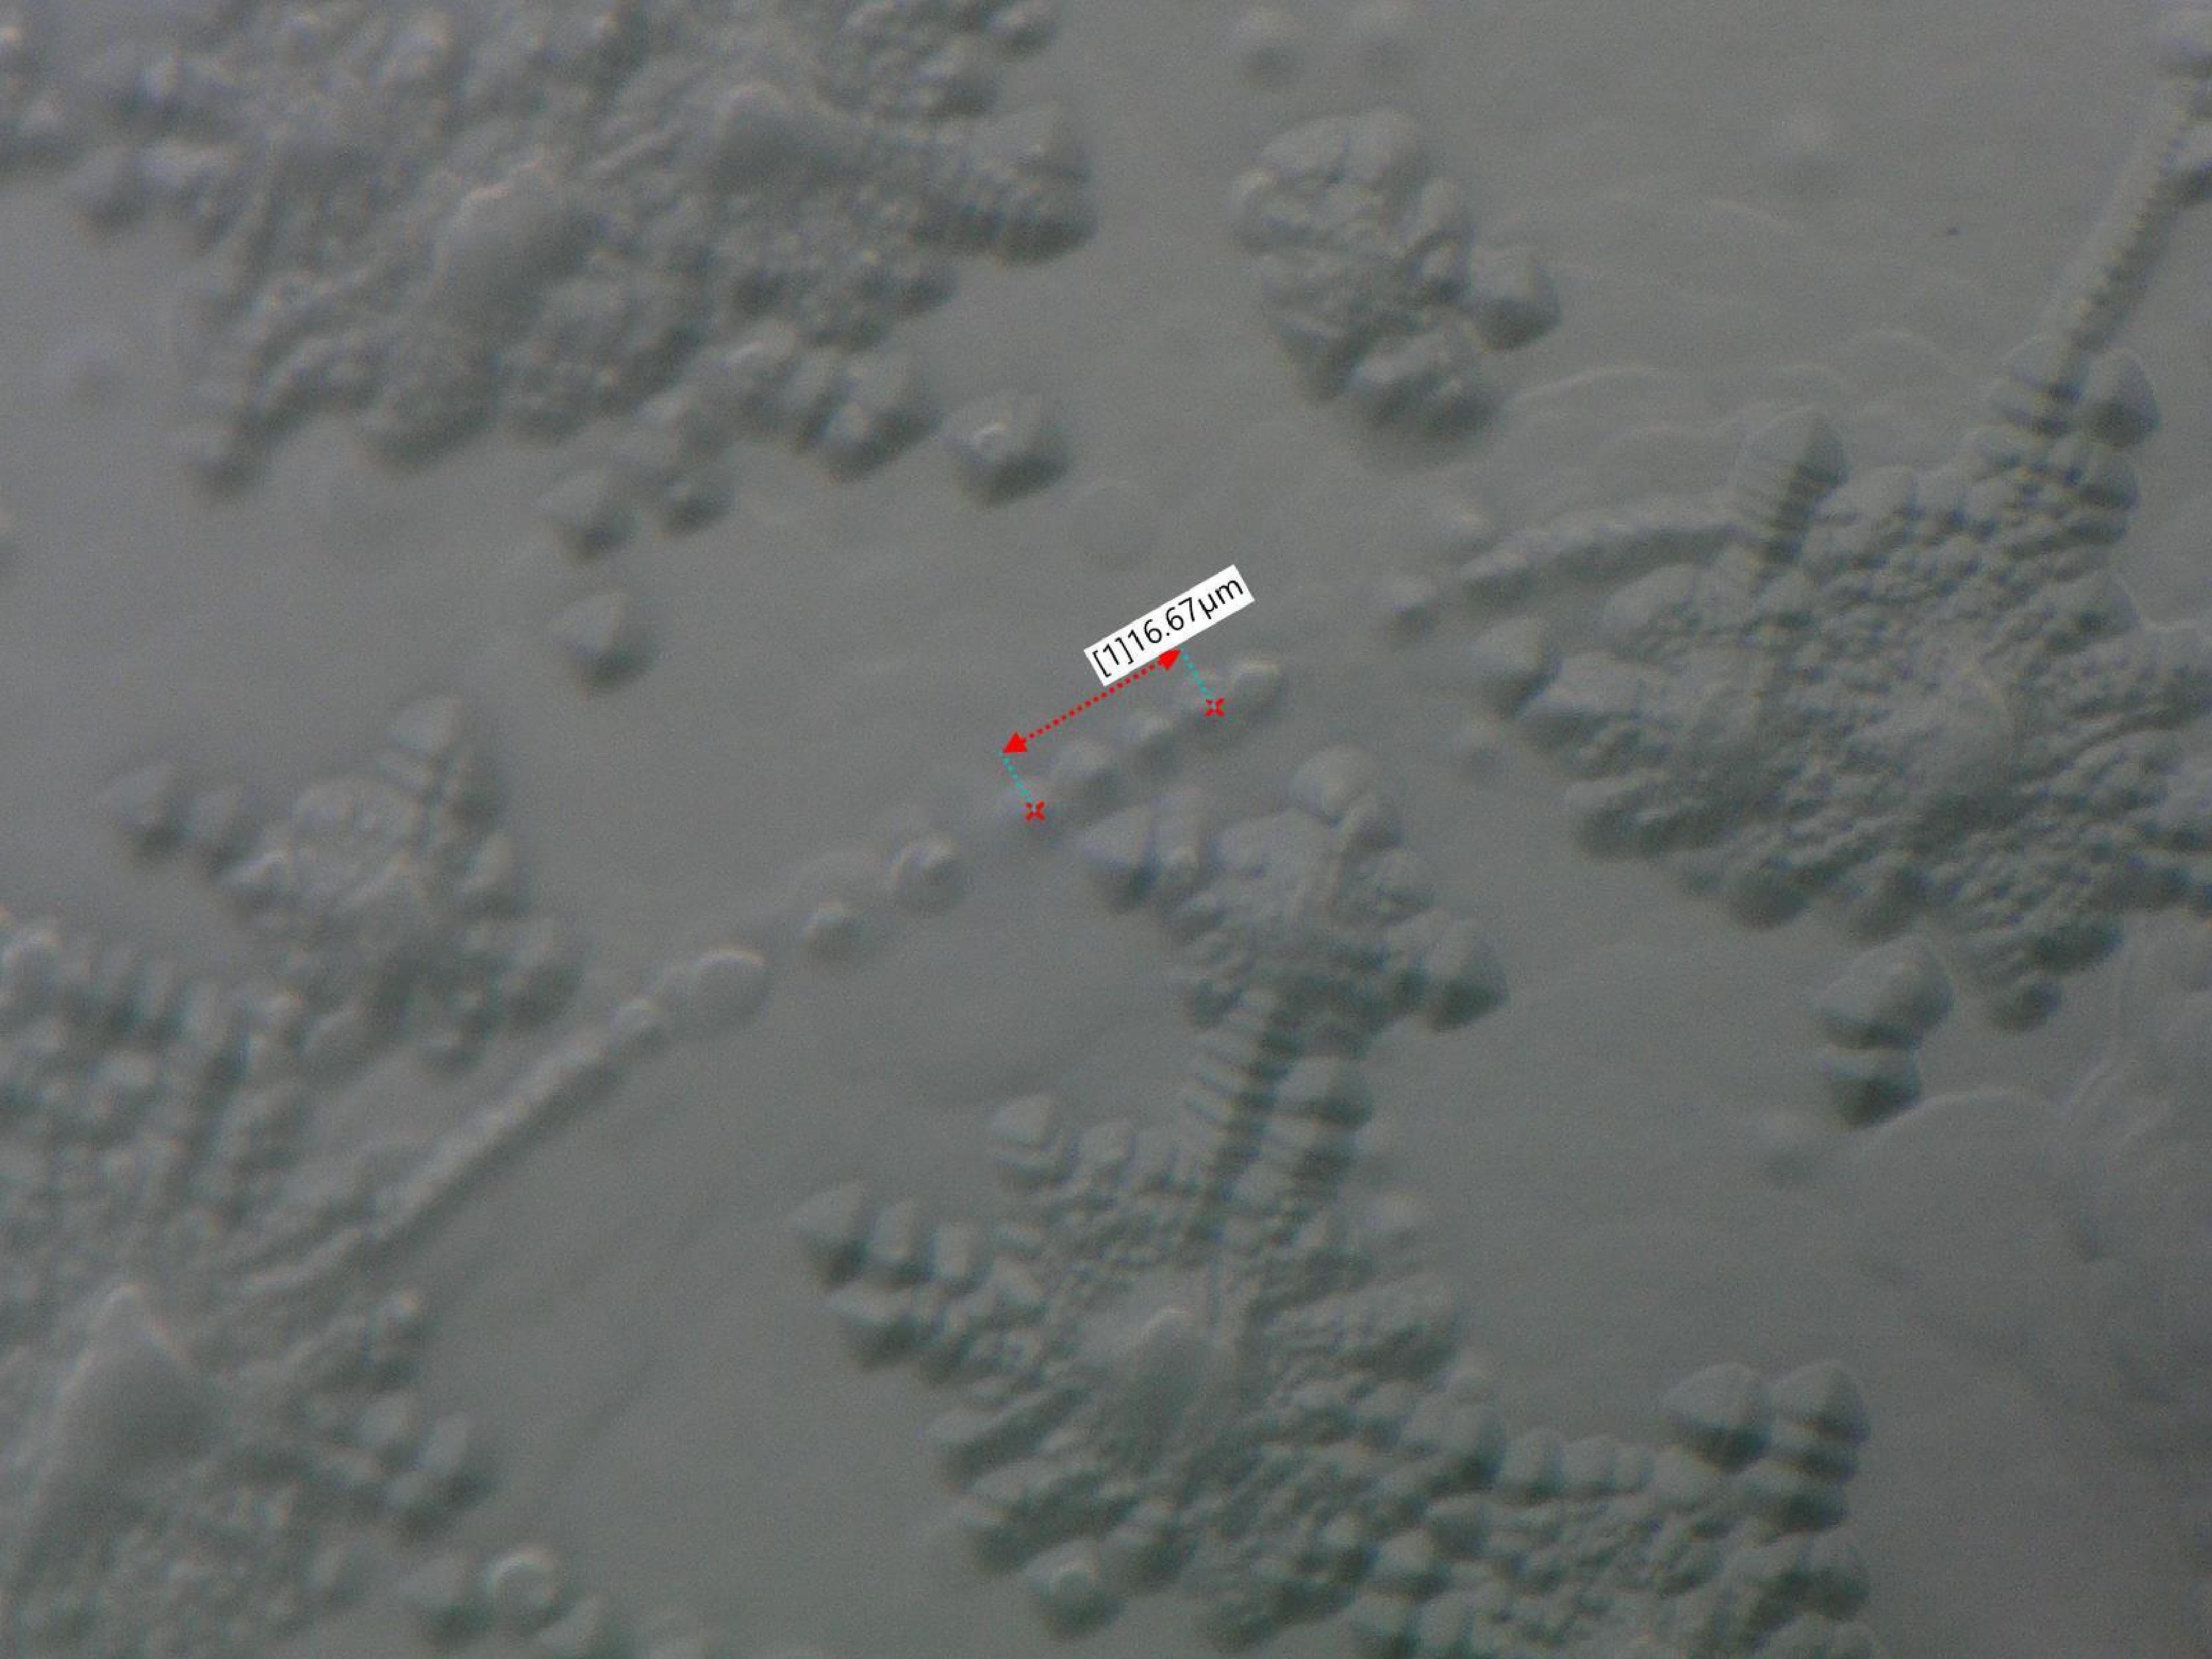
\includegraphics{KWK3_tempered.pdf}
\caption{Abb. 7}
\end{figure}

Erneut werden der Abstand zweier Ätzgrübchen \(d_2\) sowie der Winkel
\(\theta_2\) analog bestimmt. \[
\begin{eqnarray}
    d_3 &=& (5.587 \pm 0.003) \mathrm{\, \mu m} \\
    \theta_3 &=& (5.088 \pm 0.003) \mathrm{\, rad} \\
        &=& (2.915 \pm 0.002) \cdot 10^{-3\ \circ} \\
\end{eqnarray}
\]

\hypertarget{diskussion-1}{%
\paragraph{Diskussion}\label{diskussion-1}}

Alle drei ermittelten Kleinwinkelkorngrenzen auf der getemperten Probe
hatten einen Winkel im Bereich von einigen Milligrad. Damit fallen sie
alle deutlich in den Bereich einer Kleinwinkelkorngrenze, wodurch die
hier getätigte Kleinwinkelannahme gerechtfertigt ist.

\hypertarget{nadeldruckrosetten-1}{%
\subsubsection{Nadeldruckrosetten}\label{nadeldruckrosetten-1}}

\hypertarget{versetzungswanderung}{%
\subsubsection{Versetzungswanderung}\label{versetzungswanderung}}

\hypertarget{schubspannung}{%
\subsubsection{Schubspannung}\label{schubspannung}}

\hypertarget{literatur}{%
\section{Literatur}\label{literatur}}

\begin{enumerate}
\def\labelenumi{\arabic{enumi}.}
\tightlist
\item
  Dislocations in Lithiumfluoride, C. Newey und R. Davidge, editiert von
  A. Bailey, Online verfügbar unter
  \url{https://ph2.uni-koeln.de/fileadmin/Lehre/PraktikumB/Dislocations_in_Lithium_Fluoride.pdf},
  1965
\item
  C. Kittel, Einführung in die Festkörperphysik, München: Oldenbourg
  Verlag, 2005
\item
  S. Hunklinger, Festkörperphysik, München: Oldenbourg Verlag, 2011
\item
  R. Gross und A. Marx, Festkörperphysik, München: Oldenbourg Verlag,
  2012
\item
  Universität zu Köln, ``Anleitung zum Versuch 2.8 Versetzungen in
  LiF'', Online verfügbar unter
  \url{https://ph2.uni-koeln.de/fileadmin/Lehre/PraktikumB/B28-LiF_tutorial_de.pdf},
  Juni 2013
\end{enumerate}

\end{document}
